\documentclass[14pt,usenames,dvipsnames,professionalfonts]{beamer}


% =======================================================================
% Packages & definitions
% =======================================================================
\usepackage[orientation=portrait,size=a3,scale=1.0,debug]{beamerposter}
%\usepackage[orientation=portrait,a0,scale=1.0,debug]{beamerposter}

% =======================================================================
%% Font packages (see http://www.ctan.org/topic/font-greek)
% =======================================================================
% \usepackage[english,greek]{babel} 
% \usepackage[utf8]{inputenc}
% %\usepackage{lmodern}     %ruins some characters (for example, \Delta in math mode)
% \usepackage{kmath,kerkis} %use kmath for better math letters!
% \usepackage[T1]{fontenc}

\usepackage{fontspec}
%\setsansfont{Liberation Serif}
%\usepackage[english]{babel} 
%\usepackage[utf8]{inputenc}
\usepackage{lmodern}
\usepackage{kmath}
%\usepackage[T1]{fontenc}

% =======================================================================
%% Other packages
% =======================================================================
\usepackage{tabularx}
\usepackage{float}
\usepackage[countmax]{subfloat}
%\usepackage{showkeys} %uncomment to use. modifies the \label,\ref,\pageref, \cite and \bibitem commands so that the `internal' key is printed.
\usepackage{fancybox}
\usepackage{subfig}
% \let\subfigure\subfloat% compatibility between subfigure and subfig packages 
\usepackage{ifthen}
\usepackage{xcolor}
\usepackage{xspace} 
\usepackage{textcomp} %for degrees symbol 
\usepackage{epsfig}
\usepackage{graphicx}
\usepackage{amsmath,amssymb}% for advanced math typesetting % amsmath provides split
\usepackage{fancyhdr} %enables use of heaters/footers
\usepackage{bibentry} % for in-line full citations
\usepackage{gensymb} %for degrees symbol
\usepackage{tcolorbox}
\usepackage{multicol}
\usepackage{multimedia} % can be used to show movies (mp4, avi, etc..) with: \movie[options]{}{film.avi}
\usepackage{kantlipsum} 
\usepackage{nicefrac}
\usepackage{eso-pic} %position logo anywhere you want
\usepackage{textcomp,mathcomp} % degrees celcius
\usepackage[weather]{ifsym} % sun symbol
\usepackage{lipsum}
\usepackage{dirtytalk}

% =======================================================================
%% TikZ packages
% =======================================================================
\usepackage{varwidth}
\usepackage{tikz}
%\usepackage{animate}
\usepackage{media9}
\usetikzlibrary{decorations.pathmorphing}
\usetikzlibrary{decorations.markings}
\usetikzlibrary{decorations.pathreplacing}
 \usetikzlibrary{decorations.text}
\usetikzlibrary{shapes}
\usetikzlibrary{patterns}
\tcbuselibrary{skins, xparse}
\usetikzlibrary{calc}
\tcbuselibrary{hooks}
%\usepackage{pgfplots,tikz}
\usetikzlibrary{automata,positioning}
\usetikzlibrary{arrows.meta}

% =======================================================================
%% Setup Hyperref package: Enables hyper-referencing 
% =======================================================================
\usepackage{hyperref}
\hypersetup{
  plainpages=false, 
  unicode=true,                      % non-Latin (e.g. Greek) characters in Acrobat bookmarks?
  pdftoolbar=false,                  % show Acrobat toolbar?
  pdfmenubar=false,                  % show Acrobat menu?
  pdffitwindow=false,                % window fit to page when opened?
  pdfstartview={FitV},               % fits the page-width to the window?
  pdftitle={Fotios Ptochos},         % title of the document
  pdfsubject={Particle Physics},     % subject of the document
  pdfcreator={Alexandros Attikis},   % creator of the document
  pdfauthor={Alexandros Attikis},    % author of the document
  pdfproducer={Beamer/LaTeX},        % producer of the document
  pdfkeywords={{Fotios}{Ptochos}{Professor}{UCY}{Physics}{HEP}{CMS}{CERN}{FNAL}}, %keywords?
  pdfnewwindow=false,                % links in new window?
  colorlinks=false,                  % false: boxed links ,  true: colored links
  linkcolor=black,                   % color of internal links
  citecolor=black,                   % color of links to bibliography
  filecolor=black,                   % color of file links
  urlcolor=black,                    % color of external links
}

%\newcommand{\en}{\selectlanguage{english}}
%\newcommand{\gr}{\selectlanguage{greek}}
\newcommand\PutLogo[3]{%
  \AtPageLowerLeft{%
    \put(\LenToUnit{#1\paperwidth},\LenToUnit{#2\paperheight}){#3}}%
}

\newcommand{\MakePosterLogos}[4]{ %%% do NOT remove '%' at line end`
  \AddToShipoutPictureFG{
    \PutLogo{0.010}{0.924}{\includegraphics[height=0.10\paperwidth,keepaspectratio]{./figures/logos/#1}}%
    \PutLogo{0.115}{0.924}{\includegraphics[height=0.10\paperwidth,keepaspectratio]{./figures/logos/#2}}%
    \PutLogo{0.785}{0.924}{\includegraphics[height=0.10\paperwidth,keepaspectratio]{./figures/logos/#3}}%
    \PutLogo{0.890}{0.924}{\includegraphics[height=0.10\paperwidth,keepaspectratio]{./figures/logos/#4}}%
%    \PutLogo{0.1}{0.925}{\includegraphics[width=0.10\paperwidth,keepaspectratio]{./figures/logos/#1}}%
%    \PutLogo{0.0}{0.925}{\includegraphics[width=0.10\paperwidth,keepaspectratio]{./figures/logos/#2}}%
%    \PutLogo{0.8}{0.925}{\includegraphics[width=0.10\paperwidth,keepaspectratio]{./figures/logos/#3}}%
%    \PutLogo{0.9}{0.925}{\includegraphics[width=0.10\paperwidth,keepaspectratio]{./figures/logos/#4}}%
  }
}

\newcommand{\MakePosterColumns}[3]{
\newlength{\ColumnWidth}
\setlength{\ColumnWidth}{0.315\paperwidth}
\begin{columns}[t]
    \begin{columns}[t,totalwidth=1.0\paperwidth] % split up that three-column-wide column
      \begin{column}{\ColumnWidth} \input{./tex/#1.tex} \end{column}
      \begin{column}{\ColumnWidth} \input{./tex/#2.tex} \end{column}
      \begin{column}{\ColumnWidth} \input{./tex/#3.tex} \end{column}    
    \end{columns}
  \end{columns}
}

% =======================================================================
% Colour definitions. See: http://en.wikipedia.org/wiki/Web_colors
% =======================================================================
\definecolor{kOldPaper}   {RGB}{231, 229, 220}
\definecolor{kOldPaperV1} {RGB}{250, 252, 243}
\definecolor{kOldPaperAlt}{RGB}{254, 241, 226}
\definecolor{kBlack}      {RGB}{  0,   0,   0}
\definecolor{kWhite}      {RGB}{255, 255, 255}
\definecolor{kPink}       {RGB}{227,  74, 147}
\definecolor{kNavyBlue}   {RGB}{ 28, 130, 185}
\definecolor{kDarkBlue}   {RGB}{  0,   0, 214}
\definecolor{kLightBlue}  {RGB}{  0,  61, 245}
\definecolor{kvLightBlue} {RGB}{  0, 184, 245}
\definecolor{kMyBlue}     {RGB}{ 51, 102, 255}
\definecolor{kHLTausBlue} {RGB}{ 11,  36, 251}
\definecolor{kBlue}   {RGB}{ 51, 102, 255}
\definecolor{kGreen}  {RGB}{ 98, 158,  31}
\definecolor{kLightGreen}{RGB}{223, 254,  191}
\definecolor{kRed}    {RGB}{220,   0,   0}
\definecolor{kOrange} {RGB}{230, 120,  20}
\definecolor{kYellow} {RGB}{255, 221,   0}
\definecolor{kBlue}   {RGB}{ 10,  50, 150}
\definecolor{kBrown}  {RGB}{120,  89,  30}
\definecolor{kPink}   {RGB}{255,   0, 128}

% =======================================================================
% Customise tcolorboxes (package "tcolorbox")
% =======================================================================
\tcbset{
    noparskip,
    coltitle  = green,
    colframe  = pink,
    colback   = orange,
    coltext   = yellow,
    fonttitle =\normalsize, 
    posterStyle/.style = {coltitle=red, colframe=brown, colback=brown, coltext=red, fonttitle = \Large},
    boxsep       = +0.20cm,   % Title Box Height
    top          = +0.50cm,   % Top Margin (from Title box line)
    bottom       = +0.00cm,   % Bottom Margin 
    left         = +0.10cm,   % Left Margin
    right        = +0.10cm,   % Right Margin
    toptitle     = +0.10cm,   % ?
    bottomtitle  = +0.10cm,   % ?
    arc          = +0.8cm,
    nobeforeafter,
    %center title,
}
    
% new tcolorbox environment
\newtcolorbox{headline}[2][]{
  coltext          = black,
  colframe         = black, %gray!50
  colback          = \MyBlockFillColorRight,
  colbacktitle     = \MyBlockTitleBoxColor,
  coltitle         = black,
  title            = #2,
  fonttitle        = \bfseries\Huge,
  boxrule          = 0pt, % border line width
  % opacityframe     = 0,   % remove box border line
  titlerule       = 1pt,
  % colbacktitle    = red!50!yellow,
  % titlerule style = black,
  titlerule style = {black, arrows = {Hooks [arc=270]-Hooks [arc=270]}},
  opacityback     = 1.0, % 1.0 means totally transparent, 0.0 means totally opaque
  top             =-0.40cm,
  bottom          = 0.00cm,
  left            = 0.05cm,
  right           = 0.05cm,
  arc             = 0.00cm, % 0.0cm for non-rounded corners!
  sharp corners,
  frame hidden,
  parbox=false,
  #1,
}

% new tcolorbox environment
\newtcolorbox{MyArticle}[2][]{
  parbox       = false,
  coltext      = black,
  colframe     = black, %gray!50, %\MyBlockFrameColorLeft,
  colback      = \MyBlockFillColorRight, %white, %\MyBlockFillColorLeft,
  colbacktitle = \MyBlockTitleBoxColor,
  coltitle     = black,
  fonttitle    = \bfseries\Huge,
  title        = {\LARGE{\bf{#2}}},  
  boxrule      = 0pt, %frame line width
  titlerule    = 0pt, %tiitle line width
  opacityback  = 1.0, % 1.0 means totally transparent, 0.0 means totally opaque
  top          = -0.20cm,
  bottom       = +0.00cm,
  left         = +0.05cm,
  right        = +0.05cm,
  arc          = +0.00cm, % 0.0cm for non-rounded corners!
  sharp corners,
  #1,
}

\newtcolorbox{MyAd}[1][]{
  parbox       = false,
  coltext      = black,
  colframe     = black, %gray!50, %\MyBlockFrameColorLeft,
  colback      = \MyBlockFillColorRight, %white, %\MyBlockFillColorLeft,
  boxrule      = 0pt, %frame line width
  opacityback  = 1.0, % 1.0 means totally transparent, 0.0 means totally opaque
  top          = -0.00cm,
  bottom       = +0.00cm,
  left         = +0.00cm,
  right        = +0.00cm,
  arc          = +0.00cm, % 0.0cm for non-rounded corners!
  sharp corners,
  #1,
}


% =======================================================================
% Block format/colour definitions
% =======================================================================
\newcommand{\CustomiseColours}[9]{
  \newcommand{\MyFontColor}{#1}
  \newcommand{\MyHeadingsColor}{#2}
  \newcommand{\MyBlockFillColorLeft}{#3}
  \newcommand{\MyBlockFrameColorLeft}{#3}
  \newcommand{\MyBlockFillColorCenter}{#4}
  \newcommand{\MyBlockFrameColorCenter}{#4}
  \newcommand{\MyBlockFillColorRight}{#5}
  \newcommand{\MyBlockFrameColorRight}{#5}
  \newcommand{\MyBlockTitleBoxColor}{#6}
  \newcommand{\MyBackgroundColour}{#7}
  \newcommand{\MyFooterFontColour}{#8}
  \newcommand{\MyFooterFillColour}{#9}
  \setbeamercolor{background canvas}{bg=\MyBackgroundColour}
  \setbeamertemplate{navigation symbols}{}
  \setbeamercolor{block title}{fg=\MyFontColor, bg=black}
  \setbeamercolor{block body} {fg=\MyBlockFillColor, bg=black} 
  \setbeamercolor{block alerted title}{fg=red, bg=pink}
  \setbeamercolor{block alerted body} {fg=red, bg=pink}
  \setbeamercolor{title in head/foot}{fg=\MyFooterFontColour, bg=\MyFooterFillColour}
}

% =======================================================================
% Footer
% =======================================================================
\setbeamercolor{title in head/foot}{fg=black, bg=\MyBackgroundColour}
\newcommand{\FooterHeight}{0.8cm}
\newcommand{\FooterBoxDepth}{0.6cm} % The depth of a box is the distance between the baseline and the bottom of the box;

% Footer
\newcommand{\SetFooterText}[1]{
  \setbeamertemplate{footline}{
    \leavevmode
    \hbox{\begin{beamercolorbox}[wd=1.0\paperwidth,ht=\FooterHeight, dp=\FooterBoxDepth, leftskip=0.01\paperwidth, rightskip=0.01\paperwidth]{title in head/foot}
        \usebeamerfont{title in head/foot}  \centering \normalsize{#1}
      \end{beamercolorbox}
    }
  }
}

% Footer (Alternative)
\newcommand{\CustomiseFooterAlt}[3]{
  \setbeamercolor{title in head/foot}{fg=#1,bg=#2}
  \setbeamertemplate{footline}{
    \leavevmode
    \hbox{\begin{beamercolorbox}[wd=1.0\paperwidth, ht=\FooterHeight, dp=\FooterBoxDepth]{title in head/foot}
        \usebeamerfont{title in head/foot}  \centering \normalsize{#3}
      \end{beamercolorbox}
    }
  }
}


% =======================================================================
% Figures
% =======================================================================
\newcommand{\oneSubFig}[3]{
  \includegraphics[width=#3\textwidth,keepaspectratio]{figures/#2}
  \label{fig:#1}
}

\newcommand{\oneFigPosterNoCaption}[3]{
  \begin{figure}[tbp]  
      \begin{columns}
        \begin{column}{0.99\textwidth}
          \centering
          \includegraphics[width=#3\textwidth,keepaspectratio]{figures/#2}
          \label{fig:#1}
        \end{column}
      \end{columns}
  \end{figure}
}


\newcommand{\oneFigPoster}[4]{
  \begin{figure}[tbp]
    \def\figurename{Εικόνα}
      \begin{columns}
        \begin{column}{0.99\textwidth}
          \centering
          \includegraphics[width=#3\textwidth,keepaspectratio]{figures/#2}
          \label{fig:#1}
        \end{column}
      \end{columns}
    \caption{#4}
  \end{figure}
}

\newcommand{\twoFigPoster}[6]{
  \begin{figure}[tbp]
    \def\figurename{Εικόνα}
      \begin{columns}
        \begin{column}{0.47\textwidth}
          \oneSubFig{#1_a}{#2}{#3}
        \end{column}
        \begin{column}{0.47\textwidth}
          \oneSubFig{#1_b}{#4}{#5}
        \end{column}
      \end{columns}
    \caption{#6}
  \end{figure}
}

\newcommand{\twoFigPosterNoCaption}[5]{
  \begin{figure}[tbp]
      \begin{columns}
        \begin{column}{0.47\textwidth}
          \oneSubFig{#1_a}{#2}{#3}
        \end{column}
        \begin{column}{0.47\textwidth}
          \oneSubFig{#1_b}{#4}{#5}
        \end{column}
      \end{columns}
  \end{figure}
}

\newcommand{\twoFigColumnsPoster}[6]{
  \begin{figure}[tbp]
    \begin{columns}
      \begin{column}{0.5\textwidth}
        \begin{tcolorbox}[posterStyle]
          \oneSubFig{#1_a}{#2}{#3}
    \end{tcolorbox}
      \end{column}
      \begin{column}{0.5\textwidth}
        \begin{tcolorbox}[posterStyle]
          \oneSubFig{#1_b}{#4}{#5}
    \end{tcolorbox}       
      \end{column}
  \end{columns}
    \caption{#6}
  \end{figure}
}

% =======================================================================
% Enumerate Customisations (TikZ)
% =======================================================================
\newcommand*\circled[2]{\tikz[baseline=(char.base)]{  \node[circle, ball color=#2, inner sep=0.1cm] (char) {\textcolor{kWhite}#1};}}
\newcommand*\rounded[2]{\tikz[baseline=(char.base)]{ \node[draw=none,ball color=#2, shade, rounded corners=3.5pt, inner sep=0.1cm] (char) {\textcolor{kWhite}{#1}};}}

%=============================================================================
%%% General Definitions
%=============================================================================
%%% My details
\newcommand{\MyInstitute}{University Of Cyprus\xspace}
\newcommand{\MyInstituteShort}{UCY\xspace}
\newcommand{\MyName}{Alexandros Attikis\xspace}
\newcommand{\MyNameShort}{A. Attikis\xspace}

% Implicit math mode columns
\newcolumntype{L}{>{$}l<{$}}
\newcolumntype{C}{>{$}c<{$}}
\newcolumntype{R}{>{$}r<{$}}
%\newdateformat{mydate}{\THEDAY\xspace \monthname[\THEMONTH]\xspace \THEYEAR}

%=============================================================================
%%% Environments
%=============================================================================
\newenvironment{TypewriterFont}{\ttfamily}{\par} %\texttt{}

%%% Re-Define name for Table Of Contents (default is "Contents")
\renewcommand{\contentsname}{Table of Contents}

%%% Define a "make list of acronyms" command, similar to \listoffigures. \listoftables etc..
\newcommand{\listofacronymsname}{List of Acronyms}{}
\newcommand{\listofacronyms}{%
  \chapter*{\listofacronymsname}%
  \addcontentsline{toc}{chapter}{\listofacronymsname}%
  \label{sec:acronyms}%
}

%%% Define new environment where the margin values are customarily redefined
\newenvironment{changemargin}[3]{
  \begin{list}{}{
      %\setlength{\topsep}{#1}
      \setlength{\topmargin}{#1}
      \setlength{\leftmargin}{#2}
      \setlength{\rightmargin}{#3}
      \setlength{\listparindent}{\parindent}
      \setlength{\itemindent}{\parindent}
      \setlength{\parsep}{\parskip}
    }
  \item[]}{\end{list}}

%=============================================================================
%%% Reference and Citations Shortcuts
%=============================================================================
% Reference
\newcommand{\refchap}[1]{Chapter~\ref{chap:#1}\xspace}
\newcommand{\refsec}[1]{Section~\ref{sec:#1}\xspace}
\newcommand{\refdisec}[2]{Sections~\ref{sec:#1} and~\ref{sec:#2}\xspace}
\newcommand{\refapp}[1]{Appendix~\ref{app:#1}\xspace}
\newcommand{\refdiapp}[2]{Appendices~\ref{app:#1} and~\ref{app:#2}\xspace}
\newcommand{\reffig}[1]{Fig.~\ref{fig:#1}\xspace}
\newcommand{\reffigplural}{Figures}
\newcommand{\refdifig}[2]{\reffigplural~\ref{fig:#1} and~\ref{fig:#2}\xspace}
\newcommand{\reftrifig}[3]{\reffigplural~\ref{fig:#1}, \ref{fig:#2}, and~\ref{fig:#3}\xspace}
\newcommand{\reffigbegin}[1]{Fig.~\ref{fig:#1}\xspace}
\newcommand{\refdifigbegin}[2]{Figs.~\ref{fig:#1} and~\ref{fig:#2}\xspace}
\newcommand{\reftrifigbegin}[3]{Figs.~\ref{fig:#1}, \ref{fig:#2}, and~\ref{fig:#3}\xspace}
\newcommand{\refsixfigbegin}[6]{Figs.~\ref{fig:#1}, \ref{fig:#2}, \ref{fig:#3}, \ref{fig:#4}, \ref{fig:#5}, and~\ref{fig:#6}\xspace}
\newcommand{\refsevenfigbegin}[7]{Figs.~\ref{fig:#1}, \ref{fig:#2}, \ref{fig:#3}, \ref{fig:#4}, \ref{fig:#5}, \ref{fig:#6}, and~\ref{fig:#7}\xspace}
\newcommand{\reftab}[1]{Table~\ref{tab:#1}\xspace}
\newcommand{\refditab}[2]{Tables~\ref{tab:#1} and~\ref{tab:#2}\xspace}
\newcommand{\refcite}[1]{Ref.~\cite{#1}\xspace}
\newcommand{\refeq}[1]{Eq.~\eqref{eq:#1}}
\newcommand{\refdieq}[2]{Eq.~\eqref{eq:#1} and \eqref{eq:#2}\xspace}
\newcommand{\reftrieq}[3]{Eq.~\eqref{eq:#1}, \eqref{eq:#2} and \eqref{eq:#3}\xspace}
\newcommand{\refeqrange}[2]{Eqs.~\eqref{eq:#1}-\eqref{eq:#2}}
\newcommand{\reffigrange}[2]{Figs.~\ref{fig:#1}-\ref{fig:#2}}
%%% Citations
\newcommand{\refdicite}[2]{Refs.~\cite{#1} and \cite{#2}\xspace}
\newcommand{\reftricite}[3]{Refs.~\cite{#1},~\cite{#2} and \cite{#3}\xspace}
\newcommand{\refquadcite}[4]{Refs.~\cite{#1},~\cite{#2},~\cite{#3} and \cite{#4}\xspace}
\newcommand{\reftrisec}[3]{Sections~\ref{sec:#1},~\ref{sec:#2} and ~\ref{sec:#3}\xspace}
\newcommand{\refquadsec}[4]{Sections~\ref{sec:#1},~\ref{sec:#2},~\ref{sec:#3} and ~\ref{sec:#4}\xspace}
\newcommand{\refsecAndPage}[1]{Section~\ref{sec:#1} on page \pageref{sec:#1}\xspace}
\newcommand{\refappAndPage}[1]{Appendix~\ref{app:#1} on page \pageref{app:#1}\xspace} 
\newcommand{\reffigAndPage}[1]{Fig.~\ref{fig:#1} on page \pageref{fig:#1}\xspace}
\newcommand{\reftabAndPage}[1]{Table~\ref{tab:#1} on page \pageref{tab:#1}\xspace}
\newcommand{\reftritab}[3]{Tables~\ref{tab:#1},~\ref{tab:#2} and~\ref{tab:#3}\xspace}
\newcommand{\refciteAndPage}[1]{Ref.~\cite{#1} on page \pageref{#1} \xspace}
\newcommand{\refeqAndPage}[1]{Eq.~\eqref{eq:#1} on page \pageref{eq:#1} \xspace}

%=============================================================================
%%% Acronyms
%=============================================================================
\newcommand{\ATLAS}{\ac{ATLAS}\xspace}
\newcommand{\IEF}{\ac{IEF}\xspace}

%============================================================================= 
%%% General symbols
%============================================================================= 
\makeatletter
\newcommand{\romanNumber}[1]{\fontfamily{roman}\selectfont\romannumeral#1\normalfont}
\newcommand{\RomanNumber}[1]{\fontfamily{roman}\selectfont\expandafter\@slowromancap\romannumeral#1@\normalfont}
\newcommand{\Tan}[1]{\ensuremath{\tan\left(#1\right)}\xspace}
\newcommand{\Cos}[1]{\ensuremath{\tan\left(#1\right)}\xspace}
\newcommand{\Sin}[1]{\ensuremath{\tan\left(#1\right)}\xspace}
\makeatother
\newcommand{\sOrder}[1]{\ensuremath{\mathcal{O}\left(#1\right)}\xspace}
\newcommand{\sOrderOf}[1]{\sOrder{#1}}
\newcommand{\abs}[1]{\absoluteValue{#1}\xspace}
\newcommand{\sign}[1]{\ensuremath{\mathrm{sgn}\left(#1\right)}\xspace}
\newcommand{\absoluteValue}[1]{\ensuremath{\lvert#1\rvert}\xspace}
\newcommand{\Units}[1]{\tag{\ensuremath{#1}} }
\newcommand{\BR}[1]{\ensuremath{\mathcal{B}\left(#1\right)}\xspace}
\newcommand{\CTau}[1]{\ensuremath{c\tau}_{#1}\xspace}
\newcommand{\XSection}{\ensuremath{\sigma}\xspace}
\newcommand{\error}[1]{\ensuremath{\sigma_{#1}}\xspace}
\newcommand{\errorPow}[2]{\ensuremath{\sigma_{#1}^{#2}}\xspace}

%%% This Ensures that two itemize environments side by side in a
%%% two-column environment are actaully top-aligned!
%%% See: http://tex.stackexchange.com/questions/22916/top-alignment-of-itemize-in-columns-of-beamer
\makeatletter
\define@key{beamerframe}{t}[true]{% top
  \beamer@frametopskip=.2cm plus .5\paperheight\relax%
  \beamer@framebottomskip=0pt plus 1fill\relax%
  \beamer@frametopskipautobreak=\beamer@frametopskip\relax%
  \beamer@framebottomskipautobreak=\beamer@framebottomskip\relax%
  \def\beamer@initfirstlineunskip{}%
}
\makeatother
%=============================================================================
%%% Kinematic Variables
%=============================================================================
\newcommand{\pT}{\ensuremath{p_{\mathrm{T}}}\xspace}
\newcommand{\pZ}{\ensuremath{p_{\mathrm{z}}}\xspace}
\newcommand{\eT}{\ensuremath{E_{\mathrm{T}}}\xspace}
\newcommand{\deltaR}{\ensuremath{\Delta \mathrm{R}}\xspace}
\newcommand{\deltaPhi}{\ensuremath{\Delta \phi}\xspace}
\newcommand{\eTVis}{\ensuremath{E_{\mathrm{T}}^{\mathrm{vis}}}\xspace}
\newcommand{\eTCorr}{\ensuremath{E_{\mathrm{T,~corr}}}\xspace}
\newcommand{\eTSub}[1]{\ensuremath{E_{\mathrm{T,~#1}}}\xspace}
\newcommand{\etaVis}{\ensuremath{\eta^{\mathrm{vis}}}\xspace}
\newcommand{\etaCorr}{\ensuremath{\eta_{\mathrm{corr}}}\xspace}
\newcommand{\etaSub}[1]{\ensuremath{\eta_{\mathrm{#1}}}\xspace}
\newcommand{\thetaCorr}{\ensuremath{\theta_{\mathrm{corr}}}\xspace}
\newcommand{\pTPow}[1]{\ensuremath{p_{\mathrm{T}}^{\mathrm{#1}}}\xspace}
\newcommand{\pZPow}[1]{\ensuremath{p_{\mathrm{z}}^{\mathrm{#1}}}\xspace}
\newcommand{\pTSub}[1]{\ensuremath{p_{\mathrm{T},~\mathrm{#1}}}\xspace}

%=============================================================================
%%% TTI WG (HLTaus)
%=============================================================================
\newcommand{\Pythia}{\text{PYTHIA}{}6\xspace}
\newcommand{\Tauola}{\text{TAUOLA}\xspace}
\newcommand{\Geant}{\text{GEANT}{}4\xspace}
\newcommand{\Madgraph}{\text{MadGraph}\xspace}
\newcommand{\Powheg}{\text{POWHEG}\xspace}
%
\newcommand{\MCTau}{\ensuremath{\mathrm{\tau}_{\mathrm{mc}}}\xspace}
\newcommand{\McVtx}{\ensuremath{\text{MC Vertex}}\xspace}
\newcommand{\MCTauVis}{\ensuremath{\mathrm{\tau}_{\mathrm{mc}}^{\mathrm{vis}}}\xspace}
\newcommand{\LOneTrigger}{\ensuremath{\text{L1 Trigger }}\xspace}
\newcommand{\LOneTauTrigger}{\ensuremath{\text{L1 Tau Trigger }}\xspace}
\newcommand{\LOneVtx}{\ensuremath{\text{L1 Vertex}}\xspace}
\newcommand{\LOneTk}{\ensuremath{\text{L1 Track}}\xspace}
\newcommand{\LOneTks}{\ensuremath{\text{L1 Tracks}}\xspace}
\newcommand{\LOnePixTk}{\ensuremath{\text{L1 Pixel Track}}\xspace}
\newcommand{\LOnePixTks}{\ensuremath{\text{L1 Pixel Tracks}}\xspace}
%\newcommand{\LOneTkTau}{\ensuremath{\text{L1 } \mathrm{\tau}_{\mathrm{tk}}}\xspace}
%\newcommand{\LOneTkTaus}{\ensuremath{\text{L1 } \mathrm{\tau}_{\mathrm{tk}}}'s\xspace}
\newcommand{\LOneTkTau}{\LOneTk--Tau\xspace}
\newcommand{\LOneTkTaus}{\LOneTk--Taus\xspace}
\newcommand{\LOneTkCluster}{\ensuremath{\text{L1 Tk Cluster}}\xspace}
\newcommand{\LOneTkClusters}{\ensuremath{\text{L1 Tk Clusters}}\xspace}
\newcommand{\LOneLdgTk}{\ensuremath{\text{L1 Tk}^{\mathrm{ldg}}}\xspace}
\newcommand{\LOneTauLdgTk}{\ensuremath{\text{L1 } \mathrm{\tau}_{\mathrm{tk}}^{\mathrm{ldg}}}\xspace}
\newcommand{\LOneCaloTau}{\ensuremath{\text{L1 Calo Tau}}\xspace}
\newcommand{\LOneCaloTaus}{\ensuremath{\text{L1 Calos Taus}}\xspace}
\newcommand{\LOneCaloTauCandidates}{\ensuremath{\mathrm{L1}} \ensuremath{\mathrm{\tau}_{\mathrm{calo}}} candidates\xspace}
%
\newcommand{\ldgtk}[1]{\ensuremath{\mathrm{ldg~\tk{{#1}}}}\xspace}
\newcommand{\Weight}[1]{\ensuremath{\mathcal{W}_{\mathrm{#1}}}\xspace}
\newcommand{\weight}[1]{\ensuremath{\mathrm{w_{\mathrm{#1}}}}\xspace}
\newcommand{\tk}[1]{\ensuremath{\mathrm{tk_{\mathrm{#1}}}}\xspace}
\newcommand{\cluster}{\ensuremath{\mathrm{cluster}}\xspace}
\newcommand{\invMass}[1]{\ensuremath{\mathrm{m\left(#1\right)}}\xspace}
\newcommand{\calo}{\ensuremath{\mathrm{calo}}\xspace}
\newcommand{\xPOCA}[1]{\ensuremath{\mathrm{x}_{\mathrm{0}}^{\mathrm{#1}}}\xspace}
\newcommand{\yPOCA}[1]{\ensuremath{\mathrm{y}_{\mathrm{0}}^{\mathrm{#1}}}\xspace}
\newcommand{\zPOCA}[1]{\ensuremath{\mathrm{z}_{\mathrm{0}}^{\mathrm{#1}}}\xspace}
\newcommand{\rPOCAVec}[1]{\ensuremath{\vec{\mathrm{r}}_{\mathrm{0}}^{\mathrm{#1}}}\xspace}
\newcommand{\dXY}[1]{\ensuremath{\mathrm{d}_{\mathrm{xy}}^{\mathrm{#1}}}\xspace}
\newcommand{\dZero}[1]{\ensuremath{\mathrm{d}_{\mathrm{0}}^{\mathrm{#1}}}\xspace}
\newcommand{\dZeroVec}[1]{\ensuremath{\vec{\mathrm{d}}_{\mathrm{0}}^{\mathrm{#1}}}\xspace}
\newcommand{\dZeroAbs}[1]{\ensuremath{\abs{\mathrm{d}_{\mathrm{0}}^{\mathrm{#1}}}}\xspace}
\newcommand{\thetaZero}[1]{\ensuremath{\mathrm{\theta}_{\mathrm{0}}^{\mathrm{#1}}}\xspace}
\newcommand{\phiZero}[1]{\ensuremath{\mathrm{\phi}_{\mathrm{0}}^{\mathrm{#1}}}\xspace}
\newcommand{\zPOCASub}[1]{\ensuremath{\mathrm{z}_{\mathrm{0,~#1}}}\xspace}
\newcommand{\zVtx}[1]{\ensuremath{\mathrm{z}_{\mathrm{vtx}}^{\mathrm{#1}}}\xspace}
\newcommand{\xPV}[1]{\ensuremath{\mathrm{x}_{\mathrm{PV}}^{\mathrm{#1}}}\xspace}
\newcommand{\yPV}[1]{\ensuremath{\mathrm{y}_{\mathrm{PV}}^{\mathrm{#1}}}\xspace}
\newcommand{\zPV}[1]{\ensuremath{\mathrm{z}_{\mathrm{PV}}^{\mathrm{#1}}}\xspace}
%\newcommand{\redChiSq}[1]{\ensuremath{\chi^{2}_{\mathrm{#1}}/\mathrm{d.o.f}}\xspace}
\newcommand{\redChiSq}[1]{\ensuremath{\chi^{2}_{\mathrm{N}{\mathrm{#1}}}}\xspace}
\newcommand{\chiSq}{\ensuremath{\chi^{2}}\xspace}
\newcommand{\NStubs}{\ensuremath{N_{\mathrm{stubs}}}\xspace}
\newcommand{\NPsStubs}{\ensuremath{N_{\mathrm{stubs}}^{\mathrm{PS}}}\xspace}
\newcommand{\SumOver}[2]{\ensuremath{\sum\limits_{\mathrm{#1}}^{\mathrm{#2}}} \xspace}
\newcommand{\RelIsoEqn}{\ensuremath{\SumOver{i}{iso-tks}\left(\frac{\mathrm{p}_{\mathrm{T}}^{\mathrm{i}}}{\mathrm{p}_{\mathrm{T}}^{\mathrm{ldg}}}\right)}\xspace}
%\newcommand{\VtxIsoEqn}{\ensuremath{\SumOver{i}{tracks} \left( \abs{\zPOCA{\tk{m}} - \zPOCA{\tk{i}}} \leq X \sCentiMeter \right) = 0}\xspace}
\newcommand{\VtxIsoEqn}{\ensuremath{\mathrm{N}_{\mathrm{iso-tks}}\left( \abs{\zPOCA{\tk{m}} - \zPOCA{\tk{i}}} \leq X \sCentiMeter \right) = 0}\xspace}
\newcommand{\VtxIsoEqnAlt}[1]{min\ensuremath{\left(\abs{\zPOCA{\tk{m}} - \zPOCA{\tk{i}}}\right) \geq #1 \sCentiMeter}\xspace}
\newcommand{\TrigProb}{\ensuremath{\mathrm{p}_{\tau}}\xspace}
\newcommand{\TrigProbPow}[1]{\ensuremath{\mathrm{p}_{\tau}^{#1}}\xspace}
\newcommand{\TrigDiProb}{\ensuremath{\mathrm{p}_{\DiTau}}\xspace}
\newcommand{\TrigDiProbSub}[1]{\ensuremath{\mathrm{p}_{\DiTau,~#1}}\xspace}
\newcommand{\TrigEff}{\ensuremath{\varepsilon_{\tau}}\xspace}
\newcommand{\TrigEffSub}[1]{\ensuremath{\varepsilon_{\tau,~#1}}\xspace}
\newcommand{\TrigEffPow}[1]{\ensuremath{\varepsilon^{#1}_{\tau}}\xspace}
\newcommand{\TrigDiEff}{\ensuremath{\varepsilon_{\DiTau}}\xspace}
\newcommand{\TrigDiEffSub}[1]{\ensuremath{\varepsilon_{\DiTau,~#1}}\xspace}
\newcommand{\TrigDiEffPow}[1]{\ensuremath{\varepsilon^{#1}_{\DiTau}}\xspace}

% Variable initialisation
\newcommand{\DefineTkTauFromCalo}[8]{
  \newcommand{\ldgTkPtMin}{#1}
  \newcommand{\tkCollectionType}{#2}
  \newcommand{\deltaRMcMatching}{#3}
  \newcommand{\sigConeDeltaR}{#4}
  \newcommand{\isoConeDeltaR}{#5}
  \newcommand{\ldgTkDeltaRCalo}{#6}
  \newcommand{\invMassMax}{#7}
  \newcommand{\deltaPOCAzMax}{#8}
}

%=============================================================================
%%% Particles: Quarks (qP) + Leptons (lP)
%=============================================================================
\newcommand{\Lepton}[1]{\ensuremath{\ell^{#1}}\xspace}
\newcommand{\Leptons}{\ensuremath{\ell = \mathrm{e}, \mu, \tau}\xspace}
\newcommand{\qQ}{\ensuremath{\mathrm{q}}} % q for quark
\newcommand{\qQdash}{\ensuremath{\mathrm{q}'}} % q for quark
\newcommand{\qAQ}{\ensuremath{\overline{\mathrm{q}}}} % anti-quark
\newcommand{\qAQdash}{\ensuremath{\overline{\mathrm{q}}'}} % anti-quark
\newcommand{\qU}{\ensuremath{\mathrm{u}}} % u for u quark
\newcommand{\qD}{\ensuremath{\mathrm{d}}} % d for d quark
\newcommand{\qC}{\ensuremath{\mathrm{c}}} % c for c quark
\newcommand{\qS}{\ensuremath{\mathrm{s}}} % s for s quark
\newcommand{\qT}{\ensuremath{\mathrm{t}}} % t for t quark
\newcommand{\qB}{\ensuremath{\mathrm{b}}} % b for b quark
\newcommand{\qAU}{\ensuremath{\overline{\mathrm{u}}}} % u for u anti-quark
\newcommand{\qAD}{\ensuremath{\overline{\mathrm{d}}}} % d for d anti-quark
\newcommand{\qAC}{\ensuremath{\overline{\mathrm{c}}}} % c for c anti-quark
\newcommand{\qAS}{\ensuremath{\overline{\mathrm{s}}}} % s for s anti-quark
\newcommand{\qAT}{\ensuremath{\overline{\mathrm{t}}}} % t for t anti-quark
\newcommand{\qAB}{\ensuremath{\overline{\mathrm{b}}}} % b for b anti-quark
\newcommand{\glu}{\ensuremath{\mathrm{g}}\xspace}
\newcommand{\Glu}{\glu}
\newcommand{\uQuark}{\ensuremath{\qU\text{-quark}}\xspace}
\newcommand{\dQuark}{\ensuremath{\qD\text{-quark}}\xspace}
\newcommand{\cQuark}{\ensuremath{\qC\text{-quark}}\xspace}
\newcommand{\sQuark}{\ensuremath{\qS\text{-quark}}\xspace}
\newcommand{\tQuark}{\ensuremath{\qT\text{-quark}}\xspace}
\newcommand{\bQuark}{\ensuremath{\qB\text{-quark}}\xspace}
\newcommand{\auQuark}{\ensuremath{\qAU\text{-quark}}\xspace}
\newcommand{\adQuark}{\ensuremath{\qAD\text{-quark}}\xspace}
\newcommand{\acQuark}{\ensuremath{\qAC\text{-quark}}\xspace}
\newcommand{\asQuark}{\ensuremath{\qAS\text{-quark}}\xspace}
\newcommand{\atQuark}{\ensuremath{\qAT\text{-quark}}\xspace}
\newcommand{\abQuark}{\ensuremath{\qAB\text{-quark}}\xspace}
\newcommand{\lL}[1]{\ensuremath{\mathrm{\ell}^{#1}}\xspace}   %lepton
\newcommand{\lE}[1]{\ensuremath{\mathrm{e}^{#1}}\xspace}      %electron
\newcommand{\lMu}[1]{\ensuremath{\mathrm{\mu}^{#1}}\xspace}   %muon
\newcommand{\lTau}[1]{\ensuremath{\mathrm{\tau}^{#1}}\xspace} %tau
\newcommand{\lNu}[1]{\ensuremath{\mathrm{\nu}_{#1}}\xspace}   %neutrino
\newcommand{\lANu}[1]{\ensuremath{\overline{\mathrm{\nu}}_{#1}}\xspace} %anti-neutrino
\newcommand{\lTauJet}{\ensuremath{\mathrm{\tau_{\textit{h}}}}\xspace}
\newcommand{\lTauJetMc}{\ensuremath{\mathrm{\tau_{\textit{h}, \mathrm{mc}}}}\xspace}
\newcommand{\jConeR}[1]{\ensuremath{\Delta\mathrm{R}_{#1}}\xspace}


%=============================================================================
%%% Particles: Mesons (\mP)
%=============================================================================
\newcommand{\mBMeson}[2]{\ensuremath{\mathrm{B}_{#1}^{#2}}\xspace}
\newcommand{\mJPsi}[1]{\ensuremath{\mathrm{J}/\hspace{-0.14em}\psi}} % J/Psi 
\newcommand{\mHadron}[1]{\ensuremath{\mathrm{h^{#1}}\xspace}} % h to represent pions and kaons
\newcommand{\mPion}[1]{\ensuremath{\mathrm{\pi^{#1}}\xspace}}
\newcommand{\mKaon}[2]{\ensuremath{\mathrm{K^{#1}_{#2}}\xspace}}
\newcommand{\mPionOrKaon}[1]{\ensuremath{\mathrm{h^{#1}}\xspace}}
\newcommand{\mRho}[1]{\ensuremath{\mathrm{\rho^{#1}}\xspace}}
\newcommand{\mAlpha}[1]{\ensuremath{\mathrm{\alpha_{1}^{#1}}\xspace}}

%=============================================================================
%%% Particles: Bosons (\bP)
%=============================================================================
\newcommand{\bPhoton}[1]{\ensuremath{\mathrm{\gamma}^{#1}}\xspace} % photon
\newcommand{\bW}[1]{\ensuremath{\mathrm{W}^{#1}}\xspace} % W
\newcommand{\bZ}[1]{\ensuremath{\mathrm{Z}^{#1}}\xspace} % Z
\newcommand{\bZPrime}[1]{\ensuremath{\mathrm{Z}^{#1\,\prime}}\xspace} % Z'
\newcommand{\bH}[1]{\ensuremath{\mathrm{H}^{#1}}\xspace}  % Higgs (H)
\newcommand{\bh}[1]{\ensuremath{\mathrm{h}^{#1}}\xspace}  % Higgs (h)
\newcommand{\bA}[1]{\ensuremath{\mathrm{A}^{#1}}\xspace}  % CP-odd Higgs (A)


%=============================================================================
%%% Particles: Pairs
%=============================================================================
\newcommand{\pTauTau}[2]{\ensuremath{\lTau{#1}\lTau{#2}}\xspace}

%=============================================================================
%%% Decay modes: Physics channels
%=============================================================================
\newcommand{\DiTau}{\ensuremath{\lTau{}\lTau{}}\xspace}
\newcommand{\WW}{\ensuremath{\bW{\pm}\bW{\mp}}\xspace}
\newcommand{\TTbar}{\ensuremath{\qT\qAT}\xspace}
\newcommand{\TTbarToBBWW}{\ensuremath{\qT\qAT \to \qB \bW{\pm} \qB \bW{\mp}}\xspace}
\newcommand{\HToTauTau}{\ensuremath{\bH{0} \to \lTau{+}\lTau{-}}\xspace}
\newcommand{\WToQQ}{\ensuremath{\bW{\pm} \to \qQ \qAQdash}\xspace}
\newcommand{\WToTauNu}{\ensuremath{\bW{\pm} \to \lTau{\pm} \lNu{\tau}}\xspace}
\newcommand{\HToTauNu}{\ensuremath{\bH{\pm} \to \lTau{\pm} \lNu{\tau}}\xspace}
%%% 1-prong tau decays
\newcommand{\TauToEle}{\ensuremath{\lTau{-}\to \lE{-} \lANu{e} \lNu{\tau} }\xspace}
\newcommand{\TauToMu}{\ensuremath{\lTau{-}\to \lMu{-} \lANu{\mu} \lNu{\tau} }\xspace}
\newcommand{\TauToOneProng}{\ensuremath{\lTau{-} \to \mHadron{-} \lNu{\tau} }\xspace}
\newcommand{\TauToOneProngRho}{\ensuremath{\lTau{-} \to \mRho{-} \lNu{\tau} \to \mHadron{-} \mPion{0} \lNu{\tau} }\xspace}
\newcommand{\TauToOneProngAlpha}{\ensuremath{\lTau{-} \to \mAlpha{-} \lNu{\tau} \to \mHadron{-} \mPion{0}  \mPion{0} \lNu{\tau} }\xspace}
\newcommand{\TauToOneProngGEThreePiZeros}{\ensuremath{\lTau{-} \to \mHadron{-} \lNu{\tau} + \geq 3\mPion{0}}\xspace}
%%% 3-prong tau decays
\newcommand{\TauToThreeProngAlpha}{\ensuremath{\lTau{-} \to \mAlpha{-} \lNu{\tau} \to \mHadron{-} \mHadron{+} \mHadron{-} \lNu{\tau} }\xspace}
\newcommand{\TauToThreeProngGEOnePiZero}{\ensuremath{\lTau{-} \to \mHadron{-} \mHadron{+} \mHadron{-} \lNu{\tau} + \geq 1\mPion{0}}\xspace}
%%% 5-prong tau decays
\newcommand{\TauToFiveProng}{\ensuremath{\lTau{-} \to \mHadron{-} \mHadron{+} \mHadron{-} \mHadron{+} \mHadron{-} \lNu{\tau} + \geq 0\mPion{0}}\xspace}
%%% Kaon tau decays 
\newcommand{\TauToKaonShort}{\ensuremath{\lTau{-} \to \mKaon{0}{S} + X}\xspace}
\newcommand{\TauToKaonLong}{\ensuremath{\lTau{-} \to \mKaon{0}{L} + X}\xspace}
%\newcommand{\TauPlusToPion}{\ensuremath{\tau^{+} \to \pi^{+} \bar{\nu}_{\tau} }\xspace}
%\newcommand{\TauMinusToPion}{\ensuremath{\tau^{-} \to \pi^{-} \nu_{\tau} }\xspace}
%\newcommand{\TaupmToPion}{\ensuremath{\tau^{\pm} \to \pi^{\pm} \nu_{\tau} }\xspace}
%\newcommand{\TauToThreeProngOnePiZero}{\ensuremath{\tau^{-} \to h^{-} h^{+} h^{-} \pi^{0} \nu_{\tau}}\xspace}


%============================================================================= 
%%% Symbols (s)
%============================================================================= 
\newcommand{\sRadiationLength}{\ensuremath{\mathrm{X}_{\mathrm{0}}}\xspace}
\newcommand{\sAbsorbtionLength}{\ensuremath{\lambda}\xspace}
\newcommand{\sAbsorbtionLengthFull}{\ensuremath{\lambda=\frac{1}{n \sigma_{\mathrm{inelastic}}}}\xspace}
\newcommand{\sMoliereRadius}{\ensuremath{\mathrm{R}_{\mathrm{m}}}\xspace}


%============================================================================= 
%%% PHYS 101 - Symbols (s)
%============================================================================= 
%\newcommand{\sUnitVector}[1]{\ensuremath{\vec{\hat{#1}}}\xspace} %no need for arrow. hat implies it (Ptochos)
\newcommand{\sUnitVector}[1]{\ensuremath{\hat{#1}}\xspace}
\newcommand{\sUnitVectorMag}[1]{\ensuremath{\abs{\sUnitVector{#1}}}\xspace}
\newcommand{\sDeltaDistance}[1]{\ensuremath{\Delta s_{#1}}\xspace}
\newcommand{\sDeltaDistancePow}[2]{\ensuremath{\Delta s_{#1}^{#2}}\xspace}
\newcommand{\sCoords}[2]{\ensuremath{\left(#1 , #2 \right) }\xspace}
\newcommand{\sCoordsTwoD}[2]{\ensuremath{\left(x_{#1} , y_{#2} \right) }\xspace}
\newcommand{\sCoordsRelativityTwoD}[2]{\ensuremath{\left(t_{#1} , x_{#2} \right) }\xspace}
\newcommand{\sLorentzFactor}{\ensuremath{\gamma}\xspace}
\newcommand{\sLorentzFactorPow}[1]{\ensuremath{\gamma^{#1}}\xspace}
\newcommand{\sRelVelocity}[1]{\ensuremath{\beta_{#1}}\xspace}
\newcommand{\sRelVelocityPow}[2]{\ensuremath{\beta_{#1}^{#2}}\xspace}
\newcommand{\sSpeedOfLight}{\ensuremath{c}\xspace}
\newcommand{\sGravitationalConstant}{\ensuremath{G}\xspace}
\newcommand{\sSpeedOfLightPow}[1]{\ensuremath{c^{#1}}\xspace}
\newcommand{\sDensity}[1]{\ensuremath{\rho_{#1}}\xspace}
\newcommand{\sMeanDensity}[1]{\ensuremath{\overline{\rho}_{#1}}\xspace}
\newcommand{\sVelocity}[1]{\ensuremath{v_{#1}}\xspace}
\newcommand{\sVelocityVec}[1]{\ensuremath{\vec{v}_{#1}}\xspace}
\newcommand{\sVelocityPow}[2]{\ensuremath{v_{#1}^{#2}}\xspace}
\newcommand{\sDeltaVelocity}[1]{\ensuremath{\Delta v_{#1}}\xspace}
\newcommand{\sDeltaVelocityVec}[1]{\ensuremath{\Delta \vec{v}_{#1}}\xspace}
\newcommand{\sDeltaVelocityPow}[2]{\ensuremath{\Delta v_{#1}^{#2}}\xspace}
\newcommand{\sMeanVelocity}[1]{\ensuremath{\overline{v}_{#1}}\xspace}
\newcommand{\sMeanVelocityVec}[1]{\ensuremath{\overline{\vec{v}}_{#1}}\xspace}
\newcommand{\sXYplane}{\ensuremath{x-y}\xspace}
\newcommand{\sPosition}[1]{\ensuremath{r_{\mathrm{#1}}}\xspace}
\newcommand{\sPositionX}[1]{\ensuremath{x_{\mathrm{#1}}}\xspace}
\newcommand{\sPositionY}[1]{\ensuremath{y_{\mathrm{#1}}}\xspace}
\newcommand{\sPositionZ}[1]{\ensuremath{z_{\mathrm{#1}}}\xspace}
\newcommand{\sMomentum}[1]{\ensuremath{p_{\mathrm{#1}}}\xspace}
\newcommand{\sDeltaMomentum}[1]{\ensuremath{\Delta p_{#1}}\xspace}
\newcommand{\sMomentumVec}[1]{\ensuremath{\vec{p}_{#1}}\xspace}
\newcommand{\sMomentumPow}[2]{\ensuremath{p_{#1}^{#2}}\xspace}
\newcommand{\sDeltaMomentumVec}[1]{\ensuremath{\Delta \vec{p}_{#1}}\xspace}
\newcommand{\sDeltaMomentumPow}[2]{\ensuremath{\Delta p_{#1}^{#2}}\xspace}
\newcommand{\sPositionPow}[2]{\ensuremath{r_{#1}^{#2}}\xspace}
\newcommand{\sPositionXPow}[2]{\ensuremath{x_{#1}^{#2}}\xspace}
\newcommand{\sPositionYPow}[2]{\ensuremath{y_{#1}^{#2}}\xspace}
\newcommand{\sPositionPowX}[2]{\ensuremath{x_{#1}^{#2}}\xspace}
\newcommand{\sPositionPowY}[2]{\ensuremath{y_{#1}^{#2}}\xspace}
\newcommand{\sDeltaPosition}[1]{\ensuremath{\Delta r_{#1}}\xspace}
\newcommand{\sDeltaPositionX}[1]{\ensuremath{\Delta x_{#1}}\xspace}
\newcommand{\sDeltaPositionPow}[2]{\ensuremath{\Delta x_{#1}^{#2}}\xspace}
\newcommand{\sDeltaPositionPowX}[2]{\ensuremath{\Delta x_{#1}^{#2}}\xspace}
\newcommand{\sDeltaPositionY}[1]{\ensuremath{\Delta y_{#1}}\xspace}
\newcommand{\sDeltaPositionPowY}[2]{\ensuremath{\Delta y_{#1}^{#2}}\xspace}
\newcommand{\sTime}[1]{\ensuremath{t_{#1}}\xspace}
\newcommand{\sMeanTime}[1]{\ensuremath{\overline{t}_{#1}}\xspace}
\newcommand{\sTimePow}[2]{\ensuremath{t_{#1}^{#2}}\xspace}
\newcommand{\sDeltaTime}[1]{\ensuremath{\Delta t_{#1}}\xspace}
\newcommand{\sDeltaTimePow}[2]{\ensuremath{\Delta t_{#1}^{#2}}\xspace}
\newcommand{\sAcceleration}[1]{\ensuremath{a_{#1}}\xspace}
\newcommand{\sAccelerationVec}[1]{\ensuremath{\vec{a}_{#1}}\xspace}
\newcommand{\sAccelerationPow}[2]{\ensuremath{a_{#1}^{#2}}\xspace}
\newcommand{\sGravity}[1]{\ensuremath{g_{#1}}\xspace}
\newcommand{\sGravityVec}[1]{\ensuremath{\vec{g}_{#1}}\xspace}
\newcommand{\sGravityValue}{\ensuremath{9.8 \sMeterSeconds{}{-2} }\xspace}
% Length
\newcommand{\sMeter}{\ensuremath{\xspace\text{m}}\xspace}
\newcommand{\sMeterPow}[2]{\ensuremath{\xspace\text{m}_{#1}^{#2}}\xspace}
\newcommand{\sKiloMeter}{\ensuremath{\xspace\text{k\hspace{-.05em}m}}\xspace}
\newcommand{\sMilliMeter}{\ensuremath{\xspace\text{m\hspace{-.05em}m}}\xspace}
\newcommand{\sCentiMeter}{\ensuremath{\xspace\text{c\hspace{-.05em}m}}\xspace}
\newcommand{\sCentiMeterPow}[1]{\ensuremath{\xspace\text{c\hspace{-.05em}m}^{#1}}\xspace}
\newcommand{\sMicroMeter}{\ensuremath{\xspace\text{$\mu$ \hspace{-0.35em}m}}\xspace}
\newcommand{\sNanoMeter}{\ensuremath{\xspace\text{n\hspace{-.05em}m}}\xspace}
\newcommand{\sAngstrom}{\mbox{\normalfont\AA}\xspace}
%Energy
\newcommand{\sMass}[1]{\ensuremath{\xspace m_{#1}}\xspace}
\newcommand{\sMassPow}[2]{\ensuremath{\xspace m_{#1}^{#2}}\xspace}
\newcommand{\sEnergy}[1]{\ensuremath{E_{#1}}\xspace}
\newcommand{\sEnergyPow}[2]{\ensuremath{E_{#1}^{#2}}\xspace}
\newcommand{\sDeltaEnergy}[1]{\ensuremath{\Delta E_{#1}}\xspace}
\newcommand{\sPower}[1]{\ensuremath{P_{#1}}\xspace}
\newcommand{\sPowerPow}[2]{\ensuremath{P_{#1}^{#2}}\xspace}
\newcommand{\sDeltaPower}[1]{\ensuremath{\Delta P_{#1}}\xspace}
\newcommand{\sWork}[1]{\ensuremath{W_{#1}}\xspace}
\newcommand{\sDeltaWork}[1]{\ensuremath{\Delta W_{#1}}\xspace}
% Time
\newcommand{\sWattMeters}[2]{\ensuremath{\xspace \text{W}^{#1} \hspace{-.05em}\text{m}^{#2}}\xspace}
\newcommand{\sIntensity}[1]{\ensuremath{I_{#1}}\xspace}
\newcommand{\sIntensityPow}[2]{\ensuremath{I_{#1}^{#2}}\xspace}
\newcommand{\sSecond}{\ensuremath{\xspace\text{s}}}
\newcommand{\sSeconds}{\sSecond}
\newcommand{\sHour}{\ensuremath{\xspace\text{h}}}
\newcommand{\sHours}{\sHour}
\newcommand{\sYear}{\ensuremath{\xspace\text{yr}}}
\newcommand{\sYears}{\ensuremath{\xspace\text{yrs}}}
\newcommand{\sSecondPow}[1]{\ensuremath{\xspace\text{s}^{#1}}\xspace}
\newcommand{\sSecondsPow}[1]{\sSecondPow{#1}}
\newcommand{\sMilliSecond}{\ensuremath{\xspace\text{m\hspace{-.05em}s}}\xspace}
\newcommand{\sMinute}{\ensuremath{\xspace\text{min}}\xspace}
\newcommand{\sMinuteCentimeter}[2]{\ensuremath{\xspace\text{min}^{#1}\text{cm}^{#2}}\xspace}
\newcommand{\sMicroSecond}{\ensuremath{\xspace\text{$\mu$ \hspace{-0.35em}s}}\xspace}
\newcommand{\sNanoSecond}{\ensuremath{\xspace\text{n \hspace{-0.35em}s}}\xspace}
% Mass
\newcommand{\sGram}{\ensuremath{\xspace\text{\hspace{-.05em}g}}\xspace}
\newcommand{\sMilliGram}{\ensuremath{\xspace\text{m\hspace{-.05em}g}}\xspace}
\newcommand{\sKiloGram}{\ensuremath{\xspace\text{k\hspace{-.05em}g}}\xspace}
\newcommand{\sKiloGramPow}[2]{\ensuremath{\xspace\text{k\hspace{-.05em}g}_{#1}^{#2}}\xspace}
% Frequency
\newcommand{\sHz}{\ensuremath{\xspace\text{\hspace{-.05em}Hz}}\xspace}
\newcommand{\sHertz}{\sHz}
\newcommand{\skHz}{\ensuremath{\xspace\text{k\hspace{-.05em}Hz}}\xspace}
\newcommand{\sMHz}{\ensuremath{\xspace\text{M\hspace{-.05em}Hz}}\xspace}
% Force
\newcommand{\sWeight}[1]{\ensuremath{W_{#1}}\xspace}
\newcommand{\sNormal}[1]{\ensuremath{N_{#1}}\xspace}
\newcommand{\sForce}[1]{\ensuremath{F_{#1}}\xspace}
\newcommand{\sForceVec}[1]{\ensuremath{\vec{F}_{#1}}\xspace}
\newcommand{\sForceVecMag}[1]{\ensuremath{\abs{\vec{F}_{#1}}}\xspace}
\newcommand{\sMeanForce}[1]{\ensuremath{\overline{F}_{#1}}\xspace}
\newcommand{\sTension}[1]{\ensuremath{T_{#1}}\xspace}
\newcommand{\sTensionVec}[1]{\ensuremath{\vec{T}_{#1}}\xspace}
% Circular Motion
\newcommand{\sRadius}[1]{\ensuremath{r_{#1}}\xspace} %R
\newcommand{\sRadiusPow}[2]{\ensuremath{r_{#1}^{#2}}\xspace} 
\newcommand{\sDeltaRadius}[1]{\ensuremath{\Delta r_{#1}}\xspace} %R
\newcommand{\sDeltaRadiusPow}[2]{\ensuremath{\Delta r_{#1}^{#2}}\xspace} %
\newcommand{\sOmega}[1]{\ensuremath{\omega_{#1}}\xspace}
\newcommand{\sOmegaPow}[2]{\ensuremath{\omega_{#1}^{#2}}\xspace}
\newcommand{\sTheta}[1]{\ensuremath{\theta_{#1}}\xspace}
\newcommand{\sThetaPow}[2]{\ensuremath{\theta_{#1}^{#2}}\xspace}
\newcommand{\sDeltaTheta}[1]{\ensuremath{\Delta \theta_{#1}}\xspace}
\newcommand{\sPeriod}[1]{\ensuremath{T_{#1}}\xspace}
\newcommand{\sPeriodPow}[2]{\ensuremath{T_{#1}^{#2}}\xspace}
\newcommand{\sFrequency}[1]{\ensuremath{f_{#1}}\xspace}
\newcommand{\sFrequencyPow}[2]{\ensuremath{f_{#1}^{#2}}\xspace}
\newcommand{\sWavelength}[1]{\ensuremath{\lambda_{#1}}\xspace}
\newcommand{\sWavelengthPow}[2]{\ensuremath{\lambda_{#1}^{#2}}\xspace}
\newcommand{\sWavenumber}[1]{\ensuremath{k_{#1}}\xspace}
\newcommand{\sWavenumberPow}[2]{\ensuremath{k_{#1}^{#2}}\xspace}
\newcommand{\sArc}[1]{\ensuremath{s_{#1}}\xspace}
\newcommand{\sDeltaArc}[1]{\ensuremath{\Delta s_{#1}}\xspace}
% Position  vectors
\newcommand{\sPosVec}[1]{\ensuremath{\vec{r}_{#1}}\xspace}
\newcommand{\sDeltaPosVec}[1]{\ensuremath{\Delta \vec{r}_{#1}}\xspace}
% Electricity / Magnetism
\newcommand{\sElectronCharge}{\lE{}\xspace}
\newcommand{\sVolt}[1]{\ensuremath{V_{#1}}\xspace}
\newcommand{\sEField}[1]{\ensuremath{E_{#1}}\xspace}
\newcommand{\sEFieldVec}[1]{\ensuremath{\vec{E}_{#1}}\xspace}
\newcommand{\sEFieldVecMag}[1]{\ensuremath{\abs{\vec{E}_{#1}}}\xspace}
\newcommand{\sCharge}[1]{\ensuremath{q_{#1}}\xspace}
\newcommand{\sChargePow}[2]{\ensuremath{q_{#1}^{#2}}\xspace}
\newcommand{\sChargeAlt}[1]{\ensuremath{Q_{#1}}\xspace}
\newcommand{\sChargeAltPow}[2]{\ensuremath{Q_{#1}^{#2}}\xspace}
\newcommand{\sBField}[1]{\ensuremath{B_{#1}}\xspace}
\newcommand{\sBFieldPow}[2]{\ensuremath{B_{#1}^{#2}}\xspace}
\newcommand{\sBFieldVec}[1]{\ensuremath{\vec{B}_{#1}}\xspace}
\newcommand{\sBFieldVecMag}[1]{\ensuremath{\abs{\vec{B}_{#1}}}\xspace}
% Relativity
\newcommand{\sBeta}[1]{\ensuremath{\beta_{#1} }\xspace}
\newcommand{\sBetaPow}[2]{\ensuremath{\beta_{#1}^{#2}}\xspace}
%Tracker
\newcommand{\sRInv}{\ensuremath{\rho^{-1}}\xspace}
\newcommand{\sLumiUnits}{\ensuremath{\text{cm}^\text{$-$2}\,\text{s}^\text{$-$1}}\xspace}
\newcommand{\sInvFb}{\mbox{\ensuremath{\,\text{fb}^\text{$-$1}}}\xspace}
           
%============================================================================= 
%%% Units
%============================================================================= 
\newcommand{\eV}{\ensuremath{\xspace\text{eV}}\xspace}
\newcommand{\MeV}{\ensuremath{\xspace\text{MeV}}\xspace}
\newcommand{\GeV}{\ensuremath{\xspace\text{GeV}}\xspace}
\newcommand{\GeVPow}[1]{\ensuremath{\xspace\text{GeV}^{\text{#1}}}\xspace}
\newcommand{\TeVc}[1]{\ensuremath{\xspace\text{TeV}c^\text{#1}}\xspace}
\newcommand{\GeVc}[1]{\ensuremath{\xspace\text{GeV}c^\text{#1}}\xspace}
\newcommand{\MeVc}[1]{\ensuremath{\xspace\text{MeV}c^\text{#1}}\xspace}

\newcommand{\sWatt}{\ensuremath{\xspace\text{W}}\xspace}
\newcommand{\sAmpere}{\ensuremath{\xspace\text{A}}\xspace}
\newcommand{\sAmperePow}[1]{\ensuremath{\xspace\text{A}^{#1}}\xspace}
\newcommand{\sCoulomb}{\ensuremath{\xspace\text{C}}\xspace}
\newcommand{\sCoulombPow}[2]{\ensuremath{\xspace\text{C}_{#1}^{#2}}\xspace}
\newcommand{\sCoulombConstant}{\ensuremath{\xspace\text{k}_{e}}\xspace}
\newcommand{\sPlanckConstant}{\ensuremath{h}\xspace}
\newcommand{\sHBar}{\ensuremath{\hbar}\xspace}
\newcommand{\sSpringConstant}{\ensuremath{\xspace\text{k}_{\text{ελ}}}\xspace}
\newcommand{\sNewton}{\ensuremath{\xspace\text{N}}\xspace}
\newcommand{\sJoule}{\ensuremath{\xspace\text{J}}\xspace}
\newcommand{\sDegrees}{\ensuremath{^{\circ}}\xspace}
\newcommand{\sRads}{\ensuremath{\text{rads}}\xspace}
\newcommand{\sMilliRads}{\ensuremath{\xspace\text{m\hspace{-.05em}\text{rads}}}\xspace}
\newcommand{\sAU}{\ensuremath{\en\text{au} }\xspace}
\newcommand{\sEV}{\ensuremath{\xspace\text{\hspace{-.05em}eV}}\xspace}
\newcommand{\sEVC}[2]{\ensuremath{\xspace\text{\hspace{-.05em}eV}^{#1} \text{c}^{#2} }\xspace}
\newcommand{\sT}{\ensuremath{\xspace\text{T}}\xspace}
\newcommand{\sTesla}{\sT}
% Combinations
\newcommand{\sJouleSeconds}[2]{\ensuremath{\xspace\text{J}^{#1}\hspace{-.05em}\text{s}^{#2}}\xspace}
\newcommand{\sMeterSeconds}[2]{\ensuremath{\xspace\text{m}^{#1}\hspace{-.05em}\text{s}^{#2}}\xspace}
\newcommand{\sNewtonMeter}[2]{\ensuremath{\xspace\text{N}^{#1}\hspace{-.05em}\text{m}^{#2}}\xspace}
\newcommand{\sNewtonKilograms}[2]{\ensuremath{\xspace\text{N}^{#1}\hspace{-.05em}\text{kg}^{#2}}\xspace}
\newcommand{\sGramMeter}[2]{\ensuremath{\xspace\text{g}^{#1}\hspace{-.05em}\text{m}^{#2}}\xspace}
\newcommand{\sGramCentiMeter}[2]{\ensuremath{\xspace\text{g}^{#1}\hspace{-.05em}\text{cm}^{#2}}\xspace}
\newcommand{\sKilogramMeterSeconds}[3]{\ensuremath{\xspace\text{kg}^{#1}\hspace{-.05em}\text{m}^{#2}\hspace{-.05em}\text{s}^{#3}}\xspace}
\newcommand{\sKilogramMeters}[2]{\ensuremath{\xspace\text{kg}^{#1}\hstopace{-.05em}\text{m}^{#2}}\xspace}
\newcommand{\sKiloMeterHours}[2]{\ensuremath{\xspace\text{km}^{#1}\hspace{-.05em}\text{h}^{#2}}\xspace}
\newcommand{\sKiloMeterSeconds}[2]{\ensuremath{\xspace\text{km}^{#1}\hspace{-.05em}\text{s}^{#2}}\xspace}
\newcommand{\sRadSeconds}[2]{\ensuremath{\xspace\text{rad}^{#1} \text{s}^{#2}}\xspace}
\newcommand{\sNewtonMeterKilograms}[3]{\ensuremath{\xspace\text{N}^{#1}\hspace{-.05em}\text{m}^{#2}\hspace{-.05em}\text{kg}^{#3}}\xspace}
\newcommand{\sNewtonMeterKiloGram}[3]{\sNewtonMeterKilograms{#1}{#2}{#3}}
\newcommand{\sNewtonMeterCoulombs}[3]{\ensuremath{\xspace\text{N}^{#1}\hspace{-.05em}\text{m}^{#2}\hspace{-.05em}\text{C}^{#3}}\xspace}
\newcommand{\sAmpereSeconds}[2]{\ensuremath{\xspace\text{A}^{#1} \text{s}^{#2}}\xspace}
\newcommand{\sVoltMeters}[2]{\ensuremath{\xspace\text{V}^{#1} \text{m}^{#2}}\xspace}


%============================================================================= 
%%% PHYS 101 - Elements (e)
%============================================================================= 
\newcommand{\eKrypton}{\ensuremath{\tensor[_{86}]{\text{Kr}}{}}\xspace}
\newcommand{\eCaesium}{\ensuremath{\tensor[_{55}]{\text{Cs}}{}}\xspace}
\newcommand{\eLead}{\ensuremath{\tensor[_{82}]{\text{Pb}}{}}\xspace}
\newcommand{\eSilicon}{\ensuremath{\tensor[_{14}]{\text{Si}}{}}\xspace}
\newcommand{\eSiliconAlt}{Si\xspace}

%============================================================================= 
%%% Tables
%============================================================================= 
\newcommand{\HLine}{\hline}

%============================================================================= 
%%% Constants
%============================================================================= 
\newcommand{\ceV}{\ensuremath{1.6 \times 10^{-19}\sJoule}\xspace}
\newcommand{\cGravity}{\ensuremath{9.8\sMeterSeconds{}{-2}}\xspace}
\newcommand{\cGravitationalConstant}{\ensuremath{6.67\times10^{-11}\sNewtonMeterKiloGram{}{2}{-2}}\xspace}
\newcommand{\cMassSun}{\ensuremath{2\times10^{30}\sKiloGram}\xspace}
\newcommand{\cMassEarth}{\ensuremath{6\times10^{24}\sKiloGram}\xspace}
\newcommand{\cMassProton}{\ensuremath{1.67\times10^{-27}\sKiloGram}\xspace}
\newcommand{\cMassElectron}{\ensuremath{9.11\times10^{-31}\sKiloGram}\xspace}
\newcommand{\cChargeElectron}{\ensuremath{1.6\times10^{-19}\sCoulomb}\xspace}
\newcommand{\cCoulombConstant}{\ensuremath{8.99\times10^{9} \sNewtonMeterCoulombs{}{2}{-2}}\xspace}
\newcommand{\cBohrRadius}{\ensuremath{0.53\times10^{-10}\sMeter}\xspace}
\newcommand{\cSpeedOfLight}{\ensuremath{3\times10^{8}\sMeterSeconds{}{-1}}\xspace}
\newcommand{\cRadiusSun}{\ensuremath{7\times10^{8}\sMeter}\xspace}
\newcommand{\cRadiusEarth}{\ensuremath{6.4\times10^{6}\sMeter}\xspace}
\newcommand{\cDistanceEarthSun}{\ensuremath{1.5\times10^{11} \sMeter}\xspace} %1AU
\newcommand{\cAU}{\cDistanceEarthSun\xspace}
\newcommand{\cPlanckConstant}{\ensuremath{6.64\times10^{-34}\sJouleSeconds{}{}}\xspace}
\newcommand{\cElectronCharge}{\ensuremath{1.602\times10^{-19}\sCoulomb}\xspace}
\newcommand{\cProtonCharge}{\cElectronCharge\xspace}
\newcommand{\cRadiusHydrogenAtom}{\ensuremath{\sRadius{} = 5.29\times10^{-11}\sMeter}\xspace}

%============================================================================= 
%%% Calculus
%============================================================================= 
\newcommand{\Derivative}[1]{\ensuremath{d#1}\xspace}
\newcommand{\DerivativeFrac}[2]{\ensuremath{\frac{d#1}{d#2}}\xspace}
\newcommand{\pDerivative}[1]{\ensuremath{\partial#1}\xspace}
\newcommand{\pDerivativeFrac}[2]{\ensuremath{\frac{\partial#1}{\partial#2}}\xspace}
\newcommand{\DerivativeSecondFrac}[2]{\ensuremath{\frac{d^{2}#1}{d#2^{2}}}\xspace}
\newcommand{\TimeFunc}[1]{\ensuremath{#1\left(t\right)}\xspace}
\newcommand{\TimeFuncSub}[2]{\ensuremath{#1_{#2}\left(t\right)}\xspace}
\newcommand{\TimeDerivative}[1]{\ensuremath{\dot{#1}\left(t\right)}\xspace}          %Newton's dot notation
\newcommand{\TimeDerivativeVec}[1]{\ensuremath{\vec{\dot{#1}}\left(t\right)}\xspace} %Newton's dot notation
\newcommand{\TimeDerivativeSecond}[1]{\ensuremath{\ddot{#1}}\left(t\right)\xspace}          %Newton's dot notation
\newcommand{\TimeDerivativeSecondVec}[1]{\ensuremath{\vec{\ddot{#1}}\left(t\right)}\xspace} %Newton's dot notation
\newcommand{\Func}[4]{\ensuremath{#1_{#3}^{#4}\left(#2\right)}\xspace}


%============================================================================= 
%%% Hyperlinks
%============================================================================= 
\newcommand{\hMCSamplesTP}[1]{\href{https://twiki.cern.ch/twiki/bin/viewauth/CMS/PdmVProductionUpgrade2014$\#$2\_Requests\_for\_the\_TTI\_Track\_Tri}{#1}}
\newcommand{\hMCSamplesFallTwentyThirteen}[1]{\href{https://cms-pdmv.cern.ch/mcm/requests?member_of_campaign=UpgFall13d&page=0}{#1}}

%============================================================================= 
%%% Matrices
%============================================================================= 
\newcommand{\IdentityMatrix}[1]{\ensuremath{\mathbb{I}_{#1}}\xspace}
\newcommand{\TransposeMatrix}[1]{\ensuremath{{#1}^{\mathrm{T}}}\xspace}
\newcommand{\AdjointMatrix}[1]{\ensuremath{adj\left(#1\right)}\xspace}
\newcommand{\DeterminantMatrix}[1]{\ensuremath{det\left(#1\right)}\xspace}
\newcommand{\InverseMatrix}[1]{\ensuremath{{#1}^{-1}}\xspace}

%=============================================================================
% Continuous and discrete random variables
%=============================================================================
\newcommand{\Expectation}[1]{\ensuremath{\text{E}\, [#1] }\xspace }
\newcommand{\Exp}[1]{\ensuremath{\overline{#1} }\xspace }
\newcommand{\mean}[1]{\ensuremath{\mu_{#1} }\xspace }
\newcommand{\Variance}[1]{\ensuremath{\text{Var}\,[#1] }\xspace}
\newcommand{\Var}[1]{\ensuremath{\sigma_{#1}^{2} }\xspace}
\newcommand{\StandDiv}[1]{\ensuremath{\text{SD\,} [#1] }\xspace}
\newcommand{\SD}[2]{\ensuremath{\sigma_{#1}^{#2} }\xspace}

\newcommand{\Covariance}[1]{\ensuremath{\text{Cov}\,[#1] }\xspace}
\newcommand{\Cov}[1]{\ensuremath{\sigma \left(#1\right)}\xspace}

\newcommand{\Correlation}[1]{\ensuremath{\rho\left(#1\right) }\xspace}
%\newcommand{\Corr}[1]{\ensuremath{\sigma \left(#1\right)}\xspace}

%=============================================================================
% Discrete random variables
%=============================================================================
% Binomial 
\newcommand{\kBnp}{\ensuremath{B_{k}\left(n, p\right)}\xspace}
\newcommand{\kBnpCustom}[2]{\ensuremath{B_{#1}\left(#2, p\right)}\xspace}
\newcommand{\kBnpFull}{\ensuremath{\nCk p^k \left(1-p\right)^{n-k}\xspace}}
\newcommand{\kBnpCustomFull}[2]{\ensuremath{\nCkCustom{#1}{#2} p^{#2} \left(1-p\right)^{#1-#2}\xspace}}
% Poisson
\newcommand{\kPlambda}{\ensuremath{P_{k}\left(\lambda\right)}\xspace}
\newcommand{\kPlambdaFull}{\ensuremath{\frac{\lambda^k \e{-\lambda}}{\Factorial{k}}}\xspace}



% =======================================================================
% Define column width and poster size
% =======================================================================
\usetheme{confposter}


% =======================================================================
% Define Colours
% =======================================================================
\CustomiseColours
    {red!50!white} % \MyFontTitleColor (?) 
    {red!30!black} % \MyHeadingsColor (?)
    {kWhite}       % \MyBlockFillColorLeft (fill color of main body in tcolorboxes)
    {kPink}        % \MyBlockFillColorCente (?)
    {kYellow}      % \MyBlockFillColorRight (?)
    {kWhite}       % \MyBlockTitleBoxColor (fill color of heading section in tcoloorboxes)
    {kWhite}       % \MyBackgroundColour (entire poster background colour. tcolorbooxes are independent)

    
% =======================================================================
% Define Footer
% =======================================================================
\CustomiseFooterAlt{kBlack}{kWhite}{some ads go here. Actual or fake vintange MPEMPA/Tocayo etc.. apple watch? iphone }
    

% =======================================================================
% Title block (logos, title, authors, institutes)
% =======================================================================
% \MakePosterLogos{logo_mc}{logo_eu}{logo_cms}{logo_ucy}
\title{The 2022 Chronicle}
\author{Fotios Ptochos\inst{1}}
\institute{\inst{1}{University of Cyprus, Nicosia, Cyprus}}
%\date{\longdate\today}
 
% =======================================================================
% Begin document
% =======================================================================
\begin{document}

%\MakePosterColumns{ColumnOne}{ColumnTwo}{ColumnThree}
\newlength{\ColumnWidth}
\setlength{\ColumnWidth}{0.315\paperwidth}



\begin{columns}[t]
    \begin{columns}[t,totalwidth=1.0\paperwidth] % split up that three-column-wide column
      \begin{column}{0.25\paperwidth} \begin{MyArticle}[enhanced, tikz={rotate=0}, width=0.25\textwidth]{Charged Higgs boson
    Hunting}
  $t\rightarrow bH^{\pm}\rightarrow \tau^{\pm} \nu_{\tau}$............................\it{25 May 2012}\newline
  $H^{\pm}\rightarrow tb$ and $H^{\pm}\rightarrow \tau\nu$..............\it{31 August 2015}\newline
  $H^{\pm} \rightarrow \tau^{\pm} \nu_{\tau}$ ................................\it{11 March 2019}\newline
  $pp\rightarrow t(b)H^{\pm} \rightarrow tb$, all-jet.......\it{21 January 2020}\newline
  $pp\rightarrow t(b)H^{\pm} \rightarrow W^{\pm}H^{0}(\tau\tau)$...............\it{4 July 2022}
  %\begin{tabular}{l l}
%  \hline
%  \bf $H^{\pm} \rightarrow \tau^{\pm} \nu_{\tau}$  & \it{11 March 2019}\\
%  \bf $H^{\pm} \rightarrow tb$, all-jet            & \it{21 January 2020}\\
%  \bf $H^{\pm} \rightarrow W^{\pm}H^{0}(\tau\tau)$ & \it{4 July 2022}\\
%  \hline
%\end{tabular}
\end{MyArticle}
% https://cms-results.web.cern.ch/cms-results/public-results/publications/HIG-11-019/index.html
% https://cms-results.web.cern.ch/cms-results/public-results/publications/HIG-14-023/index.html
% https://cms-results.web.cern.ch/cms-results/public-results/publications/HIG-18-014/index.html
% https://cms-results.web.cern.ch/cms-results/public-results/publications/HIG-18-015/index.html
% https://cms-results.web.cern.ch/cms-results/public-results/publications/HIG-21-010/index.html


\begin{comment}
\begin{multimuons-1}[enhanced, tikz={rotate=0}, width=1.0\textwidth]{\huge Charged Higgs boson Hunting}

  \Large{$t\rightarrow bH^{\pm}\rightarrow \tau^{\pm} \nu_{\tau}$}............................\it{\Large 25 May 2012}\newline
  \Large{$H^{\pm}\rightarrow tb$ and $H^{\pm}\rightarrow \tau\nu$}..............\it{\Large 31 August 2015}\newline
  \Large{$H^{\pm} \rightarrow \tau^{\pm} \nu_{\tau}$}................................\it{\Large 11 March 2019}\newline
  \Large{$pp\rightarrow t(b)H^{\pm} \rightarrow tb$, all-jet}.......\it{\Large 21 January 2020}\newline
  \Large{$pp\rightarrow t(b)H^{\pm} \rightarrow W^{\pm}H^{0}(\tau\tau)$}...............\it{\Large 4 July 2022}
\end{multimuons-1}
\end{comment}
 \end{column}
      \begin{column}{0.75\paperwidth} % new tcolorbox environment
\newtcolorbox{headline}[2][]{
  coltext      = black,
  colframe     = \MyBlockFrameColorLeft,
  colback      = \MyBlockFillColorLeft,
  colbacktitle = \MyBlockTitleBoxColor,
  coltitle     = black,
  title        = {\Huge{\textbf{#2}}},
  fonttitle    = \bfseries,
  boxrule      = 0.2cm, %frame line width
  %tikz={rotate=#3}, % manipulate the tcolorbox as a whole (in degrees)
  top=+0.0cm, bottom=+0.0cm, left=+0.05cm, right=+0.05cm,
  %enlarge top by   = +1.0cm,  %  equivalent to mdframed 'skipabove'
  %enlarge bottom by= +0.0cm,  %  equivalent to mdframed 'skipbelow'
  %enlarge left by  = +1.5cm,  
  %enlarge right by = +0.0cm, 
  opacityback=1.0, % 1.0 means totally transparent, 0.0 means totally opaque
  arc=0.0cm,        % 0.0cm for non-rounded corners!
  #1,
}

% CMS
\begin{headline}[enhanced, tikz={rotate=0}]{Fotios Ptochos Promoted to Professor!}
  \begin{multicols}{2}
    \lipsum[1]\\ 
    \lipsum[2]\\ 
    %\lipsum[3]\\ 
    % ========================
    \begin{figure}
      \begin{center}
        \vspace{-0.2in}
        \leavevmode
        \includegraphics[width=0.5\textwidth]{./figures/Fotis6.png}
      \end{center}
    \end{figure}
    % ========================
  \end{multicols}
\end{headline}
 \end{column}
    \end{columns}
  \end{columns}

\begin{columns}[t]
    \begin{columns}[t,totalwidth=1.0\paperwidth] % split up that three-column-wide column
      \begin{column}{0.35\paperwidth} % https://gitlab.cern.ch/tdr/papers/HIG-21-010/-/tree/master/
% new tcolorbox environment
\newtcolorbox{topQuark}[2][]{
  coltext      = black,
  colframe     = \MyBlockFrameColorLeft,
  colback      = \MyBlockFillColorLeft,
  colbacktitle = \MyBlockTitleBoxColor,
  coltitle     = black,
  title        = {\Large{\textbf{#2}}},
  fonttitle    = \bfseries,
  boxrule      = 0.2cm, %frame line width
  top=+0.0cm, bottom=+0.0cm, left=+0.05cm, right=+0.05cm,
  opacityback=1.0, % 1.0 means totally transparent, 0.0 means totally opaque
  arc=0.0cm,        % 0.0cm for non-rounded corners!
  #1,
}

% CMS
\begin{topQuark}[enhanced, tikz={rotate=0}]{Search for charged Higgs bosons decaying into a top and a bottom quark in the all-jet final state}
    A search for charged Higgs bosons ($H^{\pm}$) decaying into a top
    and a bottom quark in the all-jet final state is presented. The
    analysis uses LHC proton-proton collision data recorded with the
    CMS detector in 2016 at $\sqrt{s} = 13$ TeV, corresponding to an
    integrated luminosity of 35.9~$fb^{-1}$. No significant excess is
    observed above the expected background. Model-independent upper
    limits at 95$\%$ confidence level are set on the product of the
    $H^{\pm}$ production cross section and branching fraction in two
    scenarios.  For production in association with a top quark,
    limits of 21.3 to 0.007$pb$ are obtained for $H^{\pm}$ masses in the
    range of 0.2 to 3 TeV. Combining this with a search in leptonic
    final states results in improved limits of 9.25 to 0.005 $pb$. The
    complementary $s$-channel production of an $H^{\pm}$ is
    investigated in the mass range of 0.8 to 3 TeV and the
    corresponding upper limits are 4.5 to 0.023 $pb$. These results are
    interpreted using different minimal supersymmetric extensions of
    the standard model.
\end{topQuark}
\end{column} 
      \begin{column}{0.35\paperwidth}  %\begin{MyArticle}[enhanced, height=0.2\textheight,
%tikz={rotate=0}]{Physicists Find Elusive Particle Seen as Key to
%Universe}
\begin{MyArticle}[enhanced, tikz={rotate=0}, width=0.35\textwidth]{Physicists Find Elusive Particle Seen as Key to Universe}
  \begin{multicols}{2}
    Results are presented from searches for the standard model Higgs
    boson in proton–proton collisions at and 8 TeV in the Compact Muon
    Solenoid experiment at the LHC, using data samples corresponding
    to integrated luminosities of up to 5.1 fb$^{−1}$ at 7 TeV and 5.3 fb$^{−1}$
    at 8 TeV. The search is performed in five decay modes:
    $\gamma\gamma$, $ZZ$,  $\tau^{+}\tau^{-}$, and $b\bar{b}$.
    An excess of events is observed above the expected background,
    with a local significance of 5.0 standard deviations, at a mass
    near 125 GeV, signalling the production of a new particle. The
    expected significance for a standard model Higgs boson of that
    mass is 5.8 standard deviations. The excess is most significant in
    the two decay modes with the best mass resolution, $\gamma\gamma$ and $ZZ$; a
    fit to these signals gives a mass of 
    $125.3\pm0.4(\text{stat.})\pm0.5(\text{syst.}$ GeV. The decay to
    two photons indicates that the new particle is a boson with spin 
    different from one. 
    % ========================
    \begin{figure}
      \begin{center}
        \vspace{-0.2in}
        \leavevmode
        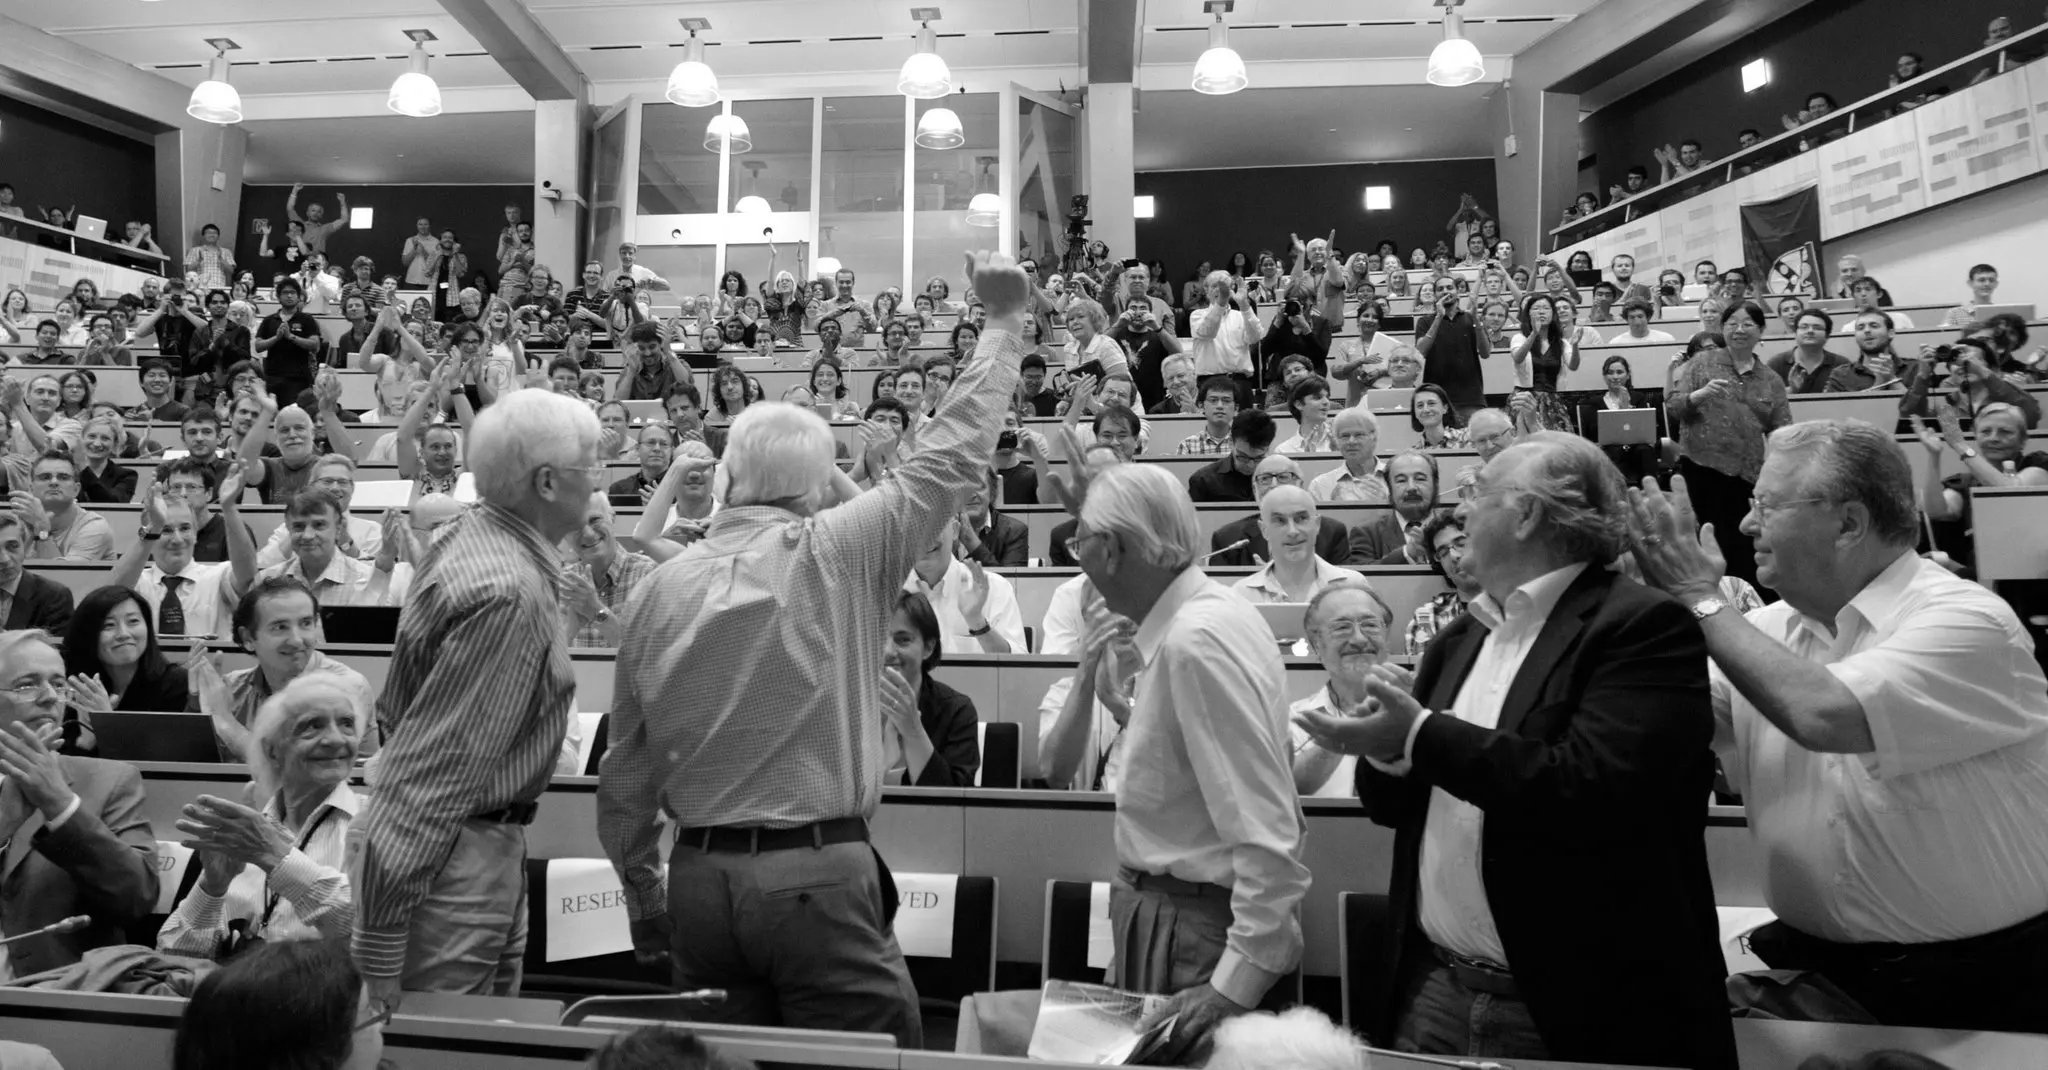
\includegraphics[width=0.5\textwidth]{./figures/HiggsBosonDiscoveryBW.png}
      \end{center}
    \end{figure}
    % ========================
  \end{multicols}
\end{MyArticle}
 \end{column}
    \end{columns}
\end{columns}

\begin{columns}[t]
  \begin{columns}[t,totalwidth=1.0\paperwidth] % split up that three-column-wide column
    \begin{column}{0.27\paperwidth} \begin{MyArticle}[enhanced, tikz={rotate=0}, boxrule=1pt,
  titlerule=0pt, width=0.33\textwidth]{CDF publishes multi-muons!}
  \begin{multicols}{2}
    We report a study of multi-muon events produced at the
    Fermilab Tevatron collider and recorded by the CDF~II detector. In a data 
    set acquired with a dedicated dimuon trigger and corresponding to an 
    integrated luminosity of 2100 pb$^{-1}$, we isolate a significant sample of 
    events in which at least one of the muon candidates is produced 
    outside of the beam pipe of radius 1.5 cm. The production cross section
    and kinematics of events in which both muon candidates are produced inside
    the beam pipe are successfully modeled by known QCD processes which
    include heavy flavor production. In contrast, we are presently unable to 
    fully account for the number and properties of the remaining events, in which
    at least one muon candidate is produced outside of the beam pipe, in terms
    of the same understanding of the CDF~II detector, trigger, and event 
    reconstruction. Several topological and kinematic properties of these 
    events are presented in this paper. These events offer a plausible 
    resolution to long-standing inconsistencies related to $b\bar{b}$
    production and decay.
    \begin{comment}
    % ========================
    \begin{figure}
      \begin{center}
        \vspace{-0.2in}
        \leavevmode
        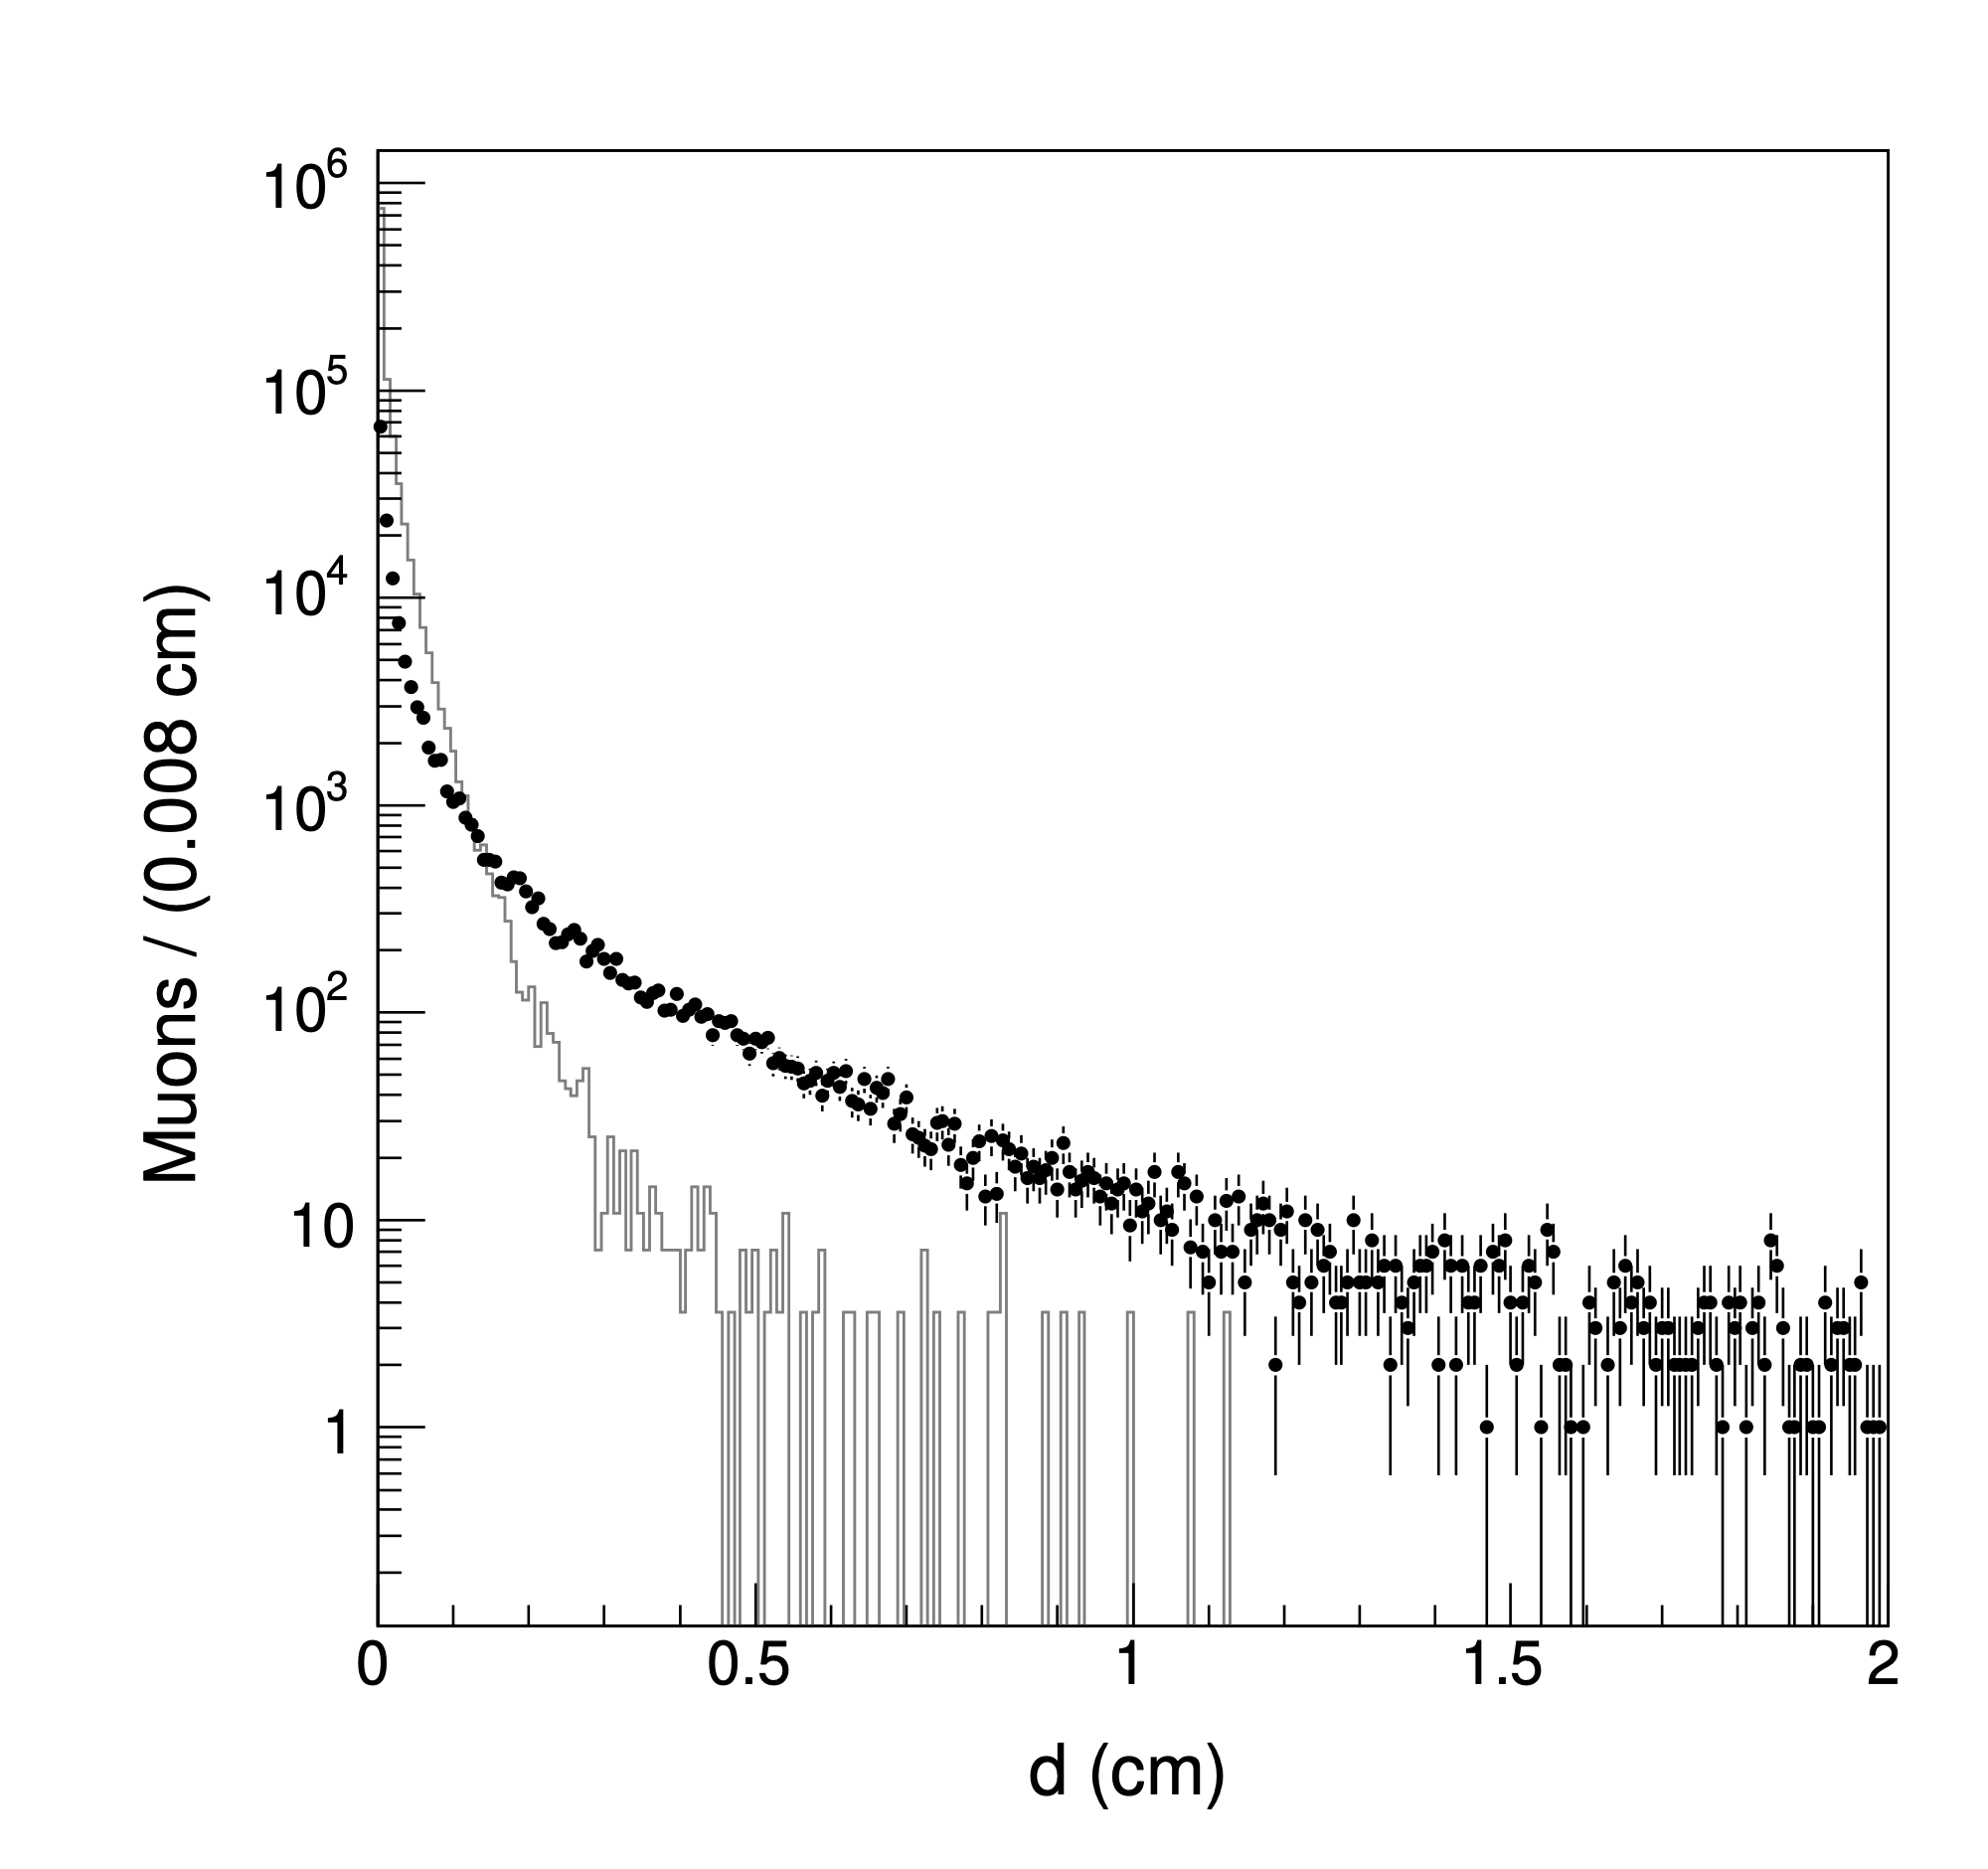
\includegraphics[width=\textwidth]{./figures/MultiMuons1BW_CDF.png}
        %\caption[] {Impact parameter distribution of muons contributed by ghost
        %  ($\bullet$) and QCD (histogram) events. Muon tracks are
        %  selected with loose SVX requirements. The detector resolution
        %  is $\simeq 30 \; \mu$m, whereas bins are 80 $\mu$m wide.} 
      \end{center}
    \end{figure}
    % ========================
    \end{comment}
  \end{multicols}
\end{MyArticle}
 \end{column}
    \begin{column}{0.27\paperwidth} % https://gitlab.cern.ch/tdr/papers/HIG-21-010/-/tree/master/
% new tcolorbox environment
\newtcolorbox{topQuark}[2][]{
  coltext      = black,
  colframe     = \MyBlockFrameColorLeft,
  colback      = \MyBlockFillColorLeft,
  colbacktitle = \MyBlockTitleBoxColor,
  coltitle     = black,
  title        = {\Large{\textbf{#2}}},
  fonttitle    = \bfseries,
  boxrule      = 0.2cm, %frame line width
  %tikz={rotate=#3}, % manipulate the tcolorbox as a whole (in degrees)
  top=+0.0cm, bottom=+0.0cm, left=+0.05cm, right=+0.05cm,
  %enlarge top by   = +1.0cm,  %  equivalent to mdframed 'skipabove'
  %enlarge bottom by= +0.0cm,  %  equivalent to mdframed 'skipbelow'
  %enlarge left by  = +1.5cm,  
  %enlarge right by = +0.0cm, 
  opacityback=1.0, % 1.0 means totally transparent, 0.0 means totally opaque
  arc=0.0cm,        % 0.0cm for non-rounded corners!
  #1,
}

% CMS
\begin{topQuark}[enhanced, tikz={rotate=0}]{Higgs boson: a tool to
    discover new physics: $H^{\pm}$}
  \begin{multicols}{2}
  A search for a charged Higgs boson $H^{\pm}$ decaying
  into a heavy neutral Higgs boson $H$ and a $W$ boson
  is presented. The analysis targets the $W$ decay into a pair
  of tau leptons with at least one of them decaying hadronically and
  with an additional electron or muon present in the event.
  The search is based on proton-proton collision data
  recorded by the CMS experiment during 2016--2018 at
  $\sqrt{s} = 13~TeV$, corresponding to an integrated
  luminosity of 138~$fb^{-1}$. The data are consistent with
  standard model background expectations. Upper limits at 95$\%$ confidence
  level are set on the product of the cross section and branching fraction
  for an $H^{\pm}$ in the mass range of 300--700 GeV, assuming an $H$ 
  with a mass of 200 GeV. The observed limits range from
  0.085 $pb$ for an $H^{\pm}$ mass of
  300 $GeV$ to 0.019~$pb$ for a mass of
  700 $GeV$. These are the first limits on $H^{\pm}$
  production in the $H^{\pm} \to H W^{\pm}$ decay channel at the LHC.
  \end{multicols}
\end{topQuark}
 \end{column}
    \begin{column}{0.4\paperwidth} \begin{MyArticle}[enhanced, tikz={rotate=0}]{Top Quark, Last Piece of Matter, Appears to Be in Place}
  \begin{multicols}{2}
    We establish the existence of the top quark using a 67 pb$^{-1}$ data
    sample of pp collisions at $\sqrt{s} = 1.8$ TeV collected with the Collider
    Detector at Fermilab (CDF). Employing techniques similar to those we
    previously published, we observe a signal consistent with $t\bar{t}$ decay to
    $WWbb$, but inconsistent with the background prediction by
    4.8$\sigma$. Additional evidence for the top quark is provided by a peak in
    the reconstructed mass distribution. We measure the top quark mass
    to be $176 \pm 8 (\text{stat.}) \pm 10 (\text{sys.})$ GeV/c$^{2}$,
    and the $t\bar{t}$ production cross section to be
    $6.8^{+3.6}_{-2.4}$ pb.
    % ========================
    \begin{figure}
      \begin{center}
        \vspace{-0.2in}
        \leavevmode
        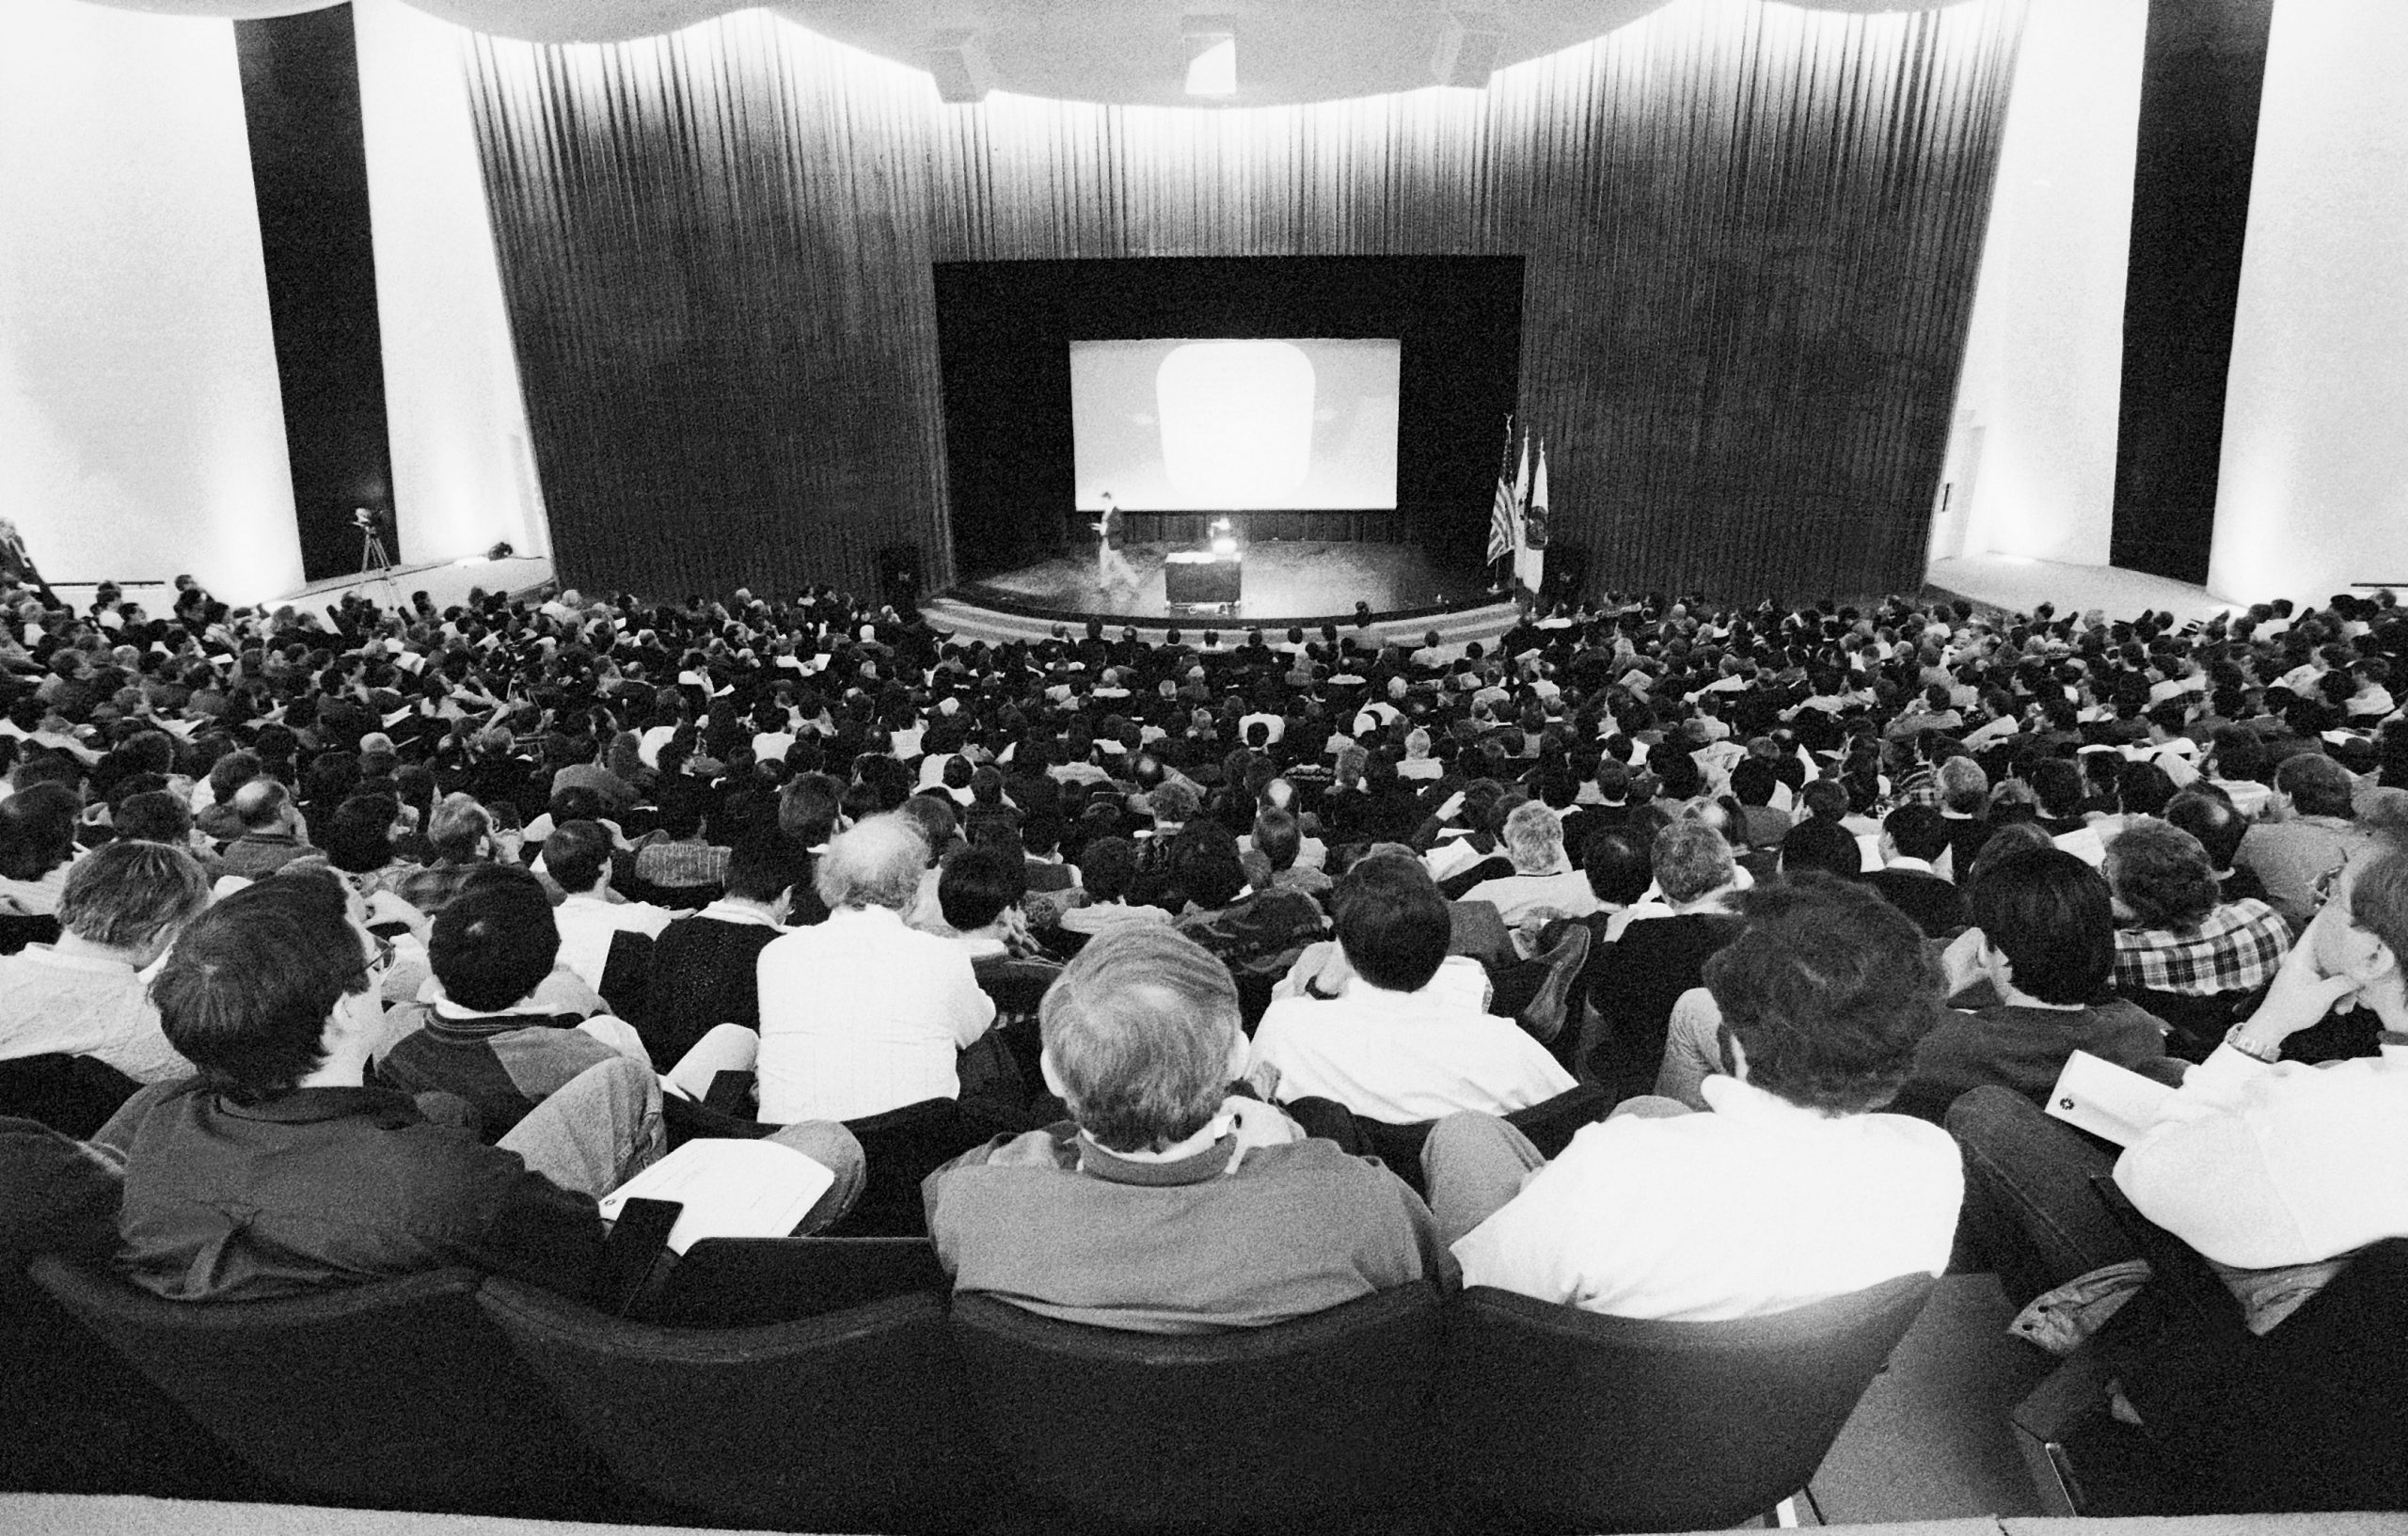
\includegraphics[width=0.5\textwidth]{./figures/TopQuarkAnnouncement.jpg}
      \end{center}
    \end{figure}
    % ========================
  \end{multicols}
\end{MyArticle}
 \begin{multimuons-2}[enhanced, tikz={rotate=0}]{Multi-Muons In CDF: The Mystery Continues}
  %\begin{multicols}{2}
    We present a phenomenological conjecture of new physics that is suggested
    by the topology and kinematic properties of the multi-muon events recently
    reported by the CDF collaboration. We show that the salient features of 
    the data can be accounted for by postulating the pair production of
    three new states $h_1$, $h_2$, and $h_3$ with masses in the range
    of 15, 7.3, and 3.6 GeV/c$^{2}$, respectively. The heavier states 
    cascade-decay into the lighter ones, whereas the lightest state 
    decays into a $\tau$ pair with a lifetime of the order of 20 ps.
    \begin{comment}
    % ========================
    \begin{figure}
      \begin{center}
        \vspace{-0.2in}
        \leavevmode
        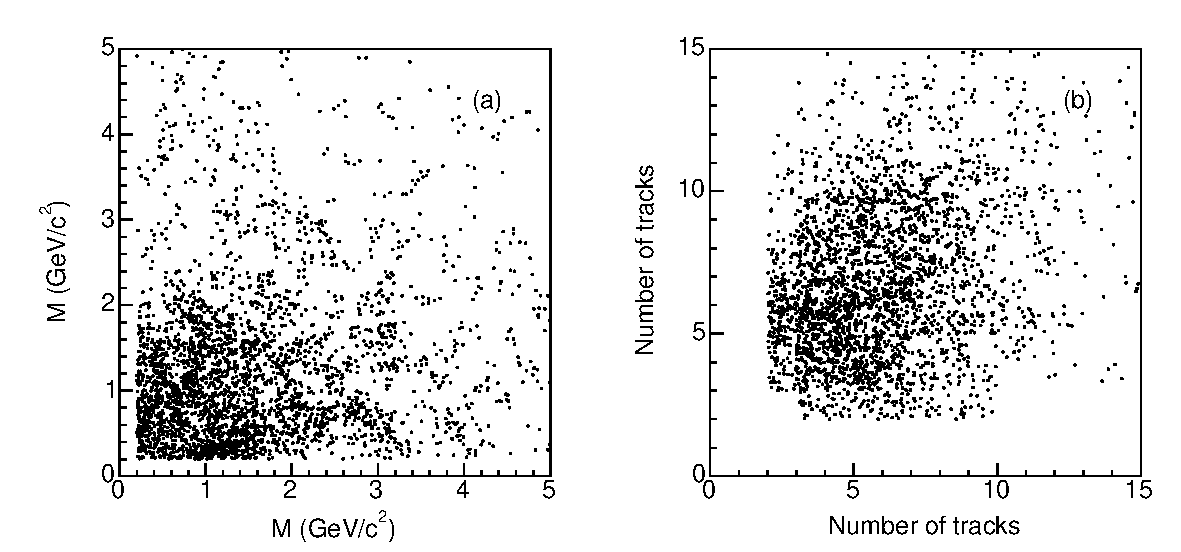
\includegraphics[width=\textwidth]{./figures/MultiMuons2_CDF.pdf}
        %\caption[]{Two-dimensional distributions, reproduced from Ref.~\cite{a0disc},
        %  of (a) the invariant mass, $M$, of all muons and (b) the total
        %  number of tracks contained in a $36.8^{\deg}$ cone when both
        %  cones contain at least two muons.}
      \end{center}
    \end{figure}
    % ========================
    \end{comment}
%  \end{multicols}
\end{multimuons-2}
\end{column}
  \end{columns}
\end{columns}

%    \begin{columns}[t]
%    \begin{columns}[t,totalwidth=1.0\paperwidth] % split up that three-column-wide column
%      \begin{column}{0.25\paperwidth} \begin{MyArticle}[enhanced, tikz={rotate=0}, boxrule=1pt,
  titlerule=0pt, width=0.33\textwidth]{CDF publishes multi-muons!}
  \begin{multicols}{2}
    We report a study of multi-muon events produced at the
    Fermilab Tevatron collider and recorded by the CDF~II detector. In a data 
    set acquired with a dedicated dimuon trigger and corresponding to an 
    integrated luminosity of 2100 pb$^{-1}$, we isolate a significant sample of 
    events in which at least one of the muon candidates is produced 
    outside of the beam pipe of radius 1.5 cm. The production cross section
    and kinematics of events in which both muon candidates are produced inside
    the beam pipe are successfully modeled by known QCD processes which
    include heavy flavor production. In contrast, we are presently unable to 
    fully account for the number and properties of the remaining events, in which
    at least one muon candidate is produced outside of the beam pipe, in terms
    of the same understanding of the CDF~II detector, trigger, and event 
    reconstruction. Several topological and kinematic properties of these 
    events are presented in this paper. These events offer a plausible 
    resolution to long-standing inconsistencies related to $b\bar{b}$
    production and decay.
    \begin{comment}
    % ========================
    \begin{figure}
      \begin{center}
        \vspace{-0.2in}
        \leavevmode
        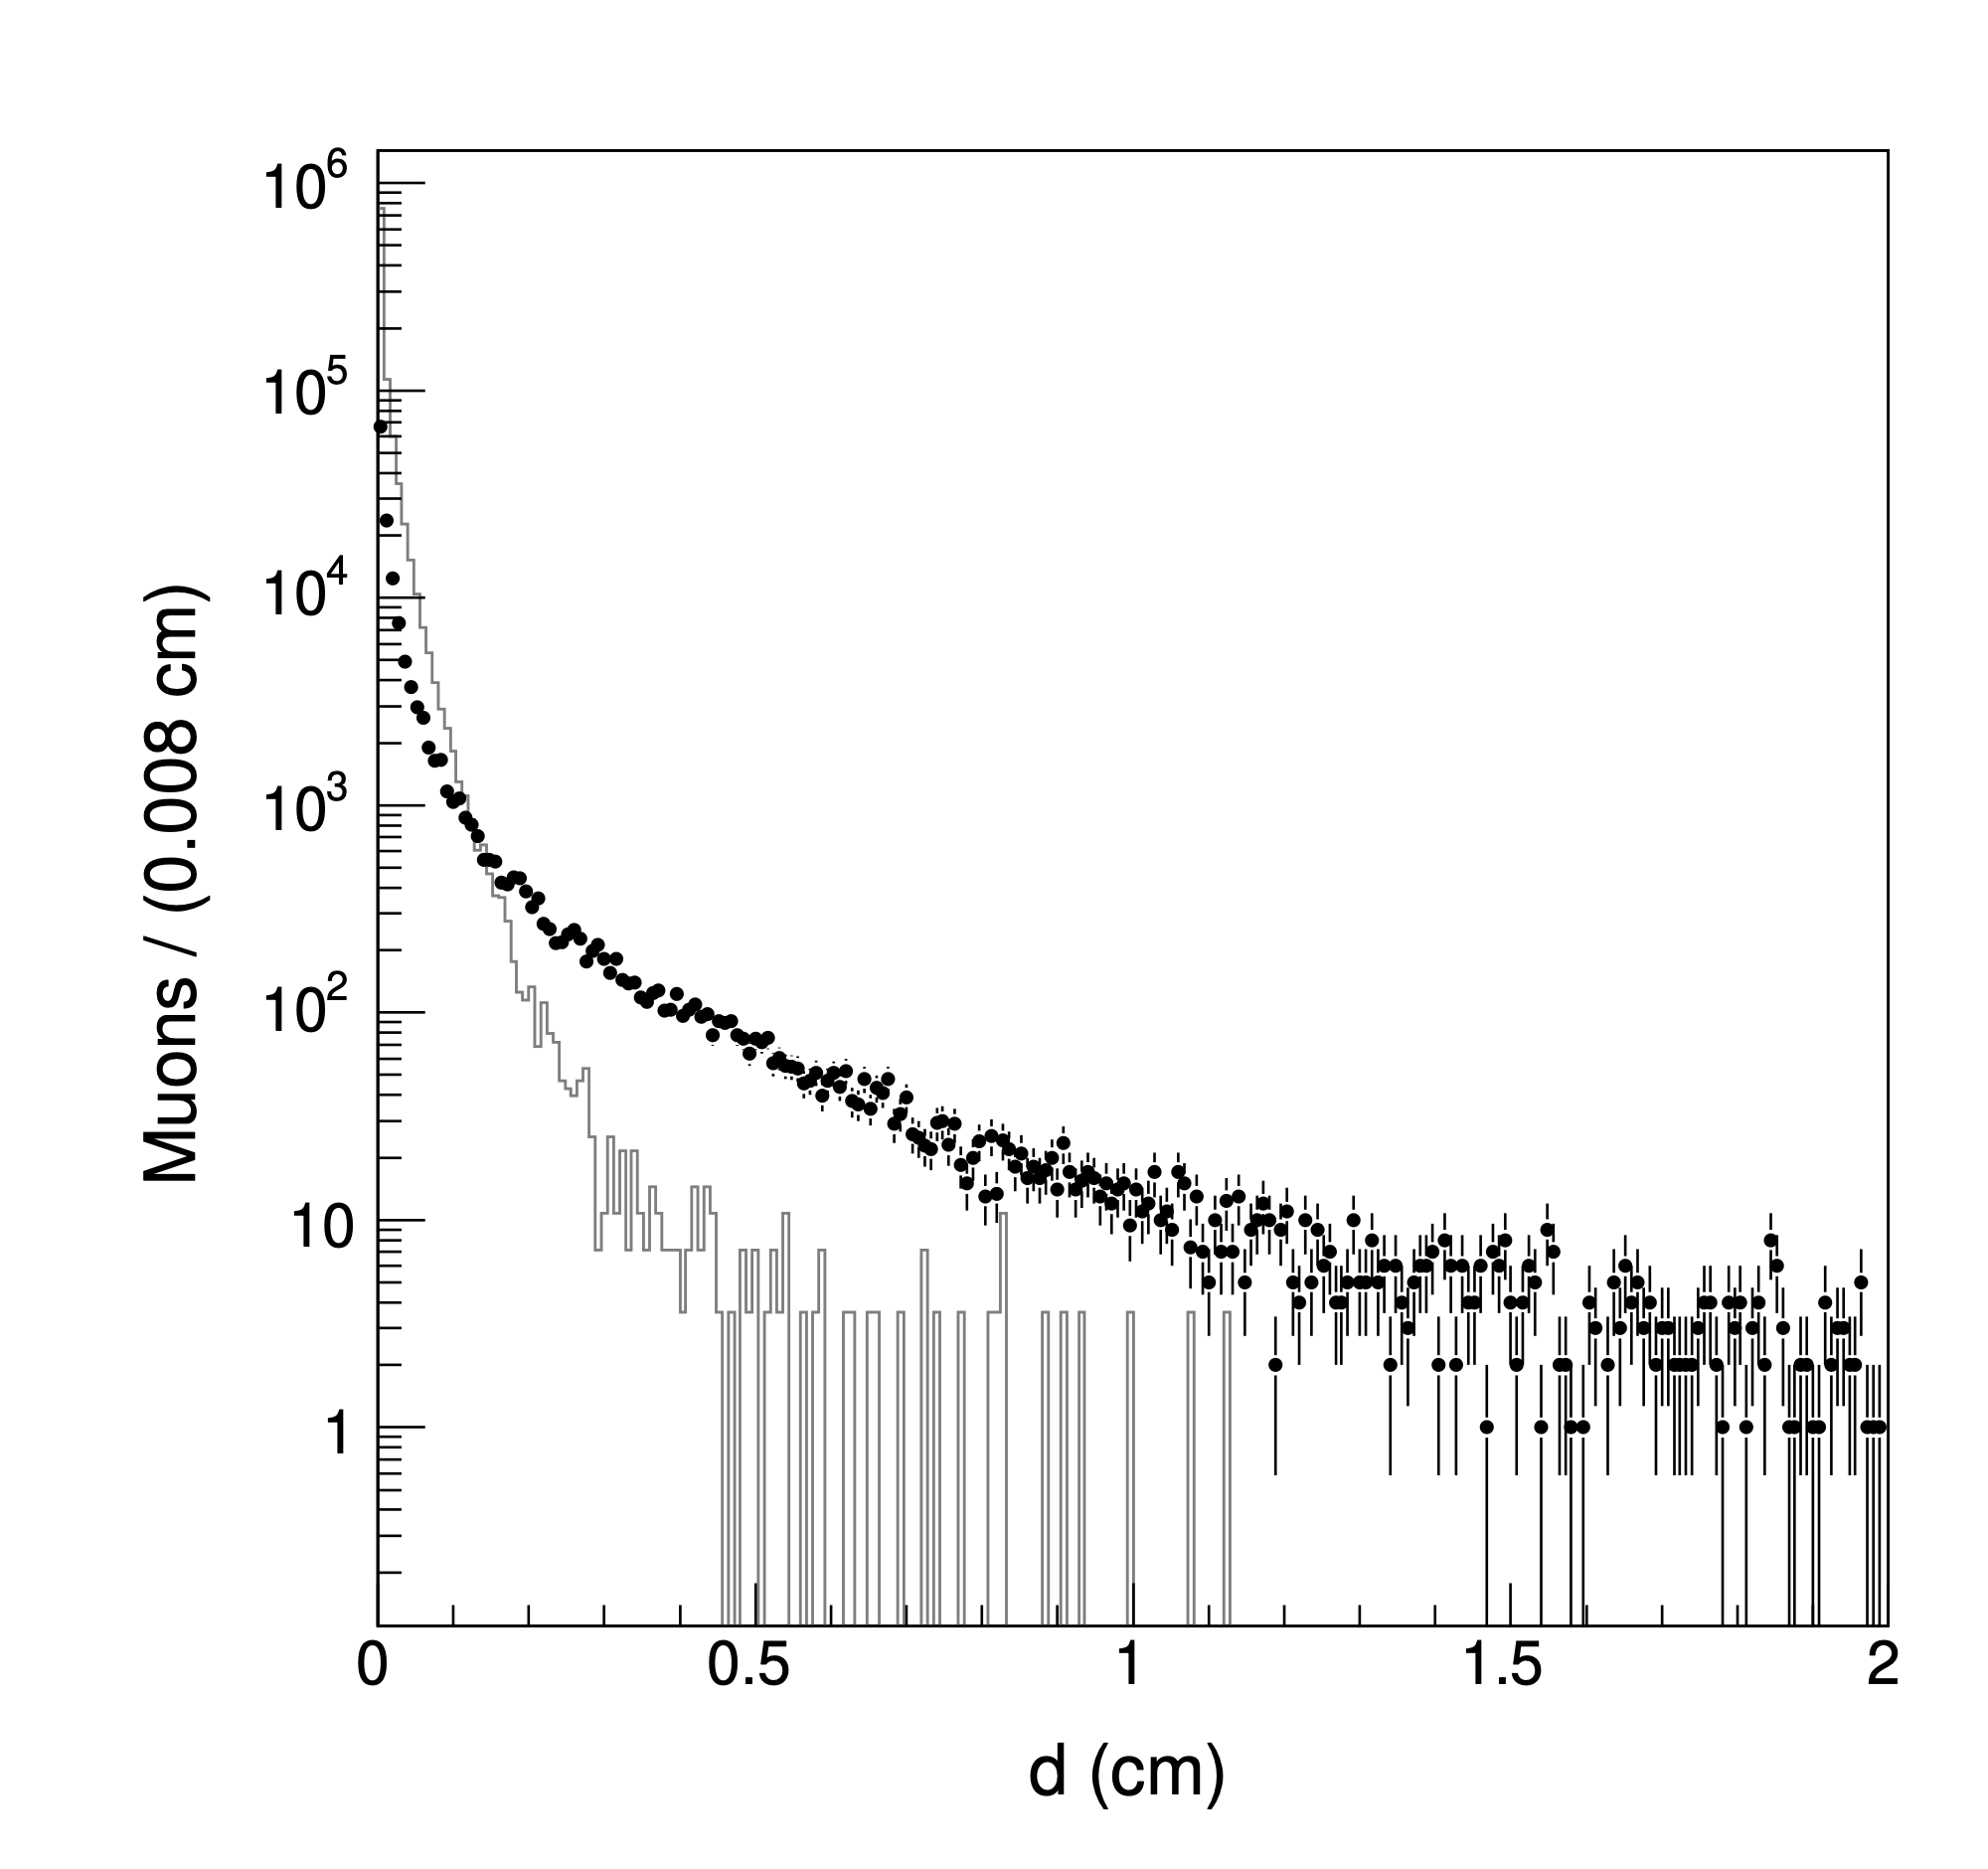
\includegraphics[width=\textwidth]{./figures/MultiMuons1BW_CDF.png}
        %\caption[] {Impact parameter distribution of muons contributed by ghost
        %  ($\bullet$) and QCD (histogram) events. Muon tracks are
        %  selected with loose SVX requirements. The detector resolution
        %  is $\simeq 30 \; \mu$m, whereas bins are 80 $\mu$m wide.} 
      \end{center}
    \end{figure}
    % ========================
    \end{comment}
  \end{multicols}
\end{MyArticle}
 \begin{MyArticle}[enhanced, tikz={rotate=0}, width=0.25\textwidth]{Charged Higgs boson
    Hunting}
  $t\rightarrow bH^{\pm}\rightarrow \tau^{\pm} \nu_{\tau}$............................\it{25 May 2012}\newline
  $H^{\pm}\rightarrow tb$ and $H^{\pm}\rightarrow \tau\nu$..............\it{31 August 2015}\newline
  $H^{\pm} \rightarrow \tau^{\pm} \nu_{\tau}$ ................................\it{11 March 2019}\newline
  $pp\rightarrow t(b)H^{\pm} \rightarrow tb$, all-jet.......\it{21 January 2020}\newline
  $pp\rightarrow t(b)H^{\pm} \rightarrow W^{\pm}H^{0}(\tau\tau)$...............\it{4 July 2022}
  %\begin{tabular}{l l}
%  \hline
%  \bf $H^{\pm} \rightarrow \tau^{\pm} \nu_{\tau}$  & \it{11 March 2019}\\
%  \bf $H^{\pm} \rightarrow tb$, all-jet            & \it{21 January 2020}\\
%  \bf $H^{\pm} \rightarrow W^{\pm}H^{0}(\tau\tau)$ & \it{4 July 2022}\\
%  \hline
%\end{tabular}
\end{MyArticle}
% https://cms-results.web.cern.ch/cms-results/public-results/publications/HIG-11-019/index.html
% https://cms-results.web.cern.ch/cms-results/public-results/publications/HIG-14-023/index.html
% https://cms-results.web.cern.ch/cms-results/public-results/publications/HIG-18-014/index.html
% https://cms-results.web.cern.ch/cms-results/public-results/publications/HIG-18-015/index.html
% https://cms-results.web.cern.ch/cms-results/public-results/publications/HIG-21-010/index.html


\begin{comment}
\begin{multimuons-1}[enhanced, tikz={rotate=0}, width=1.0\textwidth]{\huge Charged Higgs boson Hunting}

  \Large{$t\rightarrow bH^{\pm}\rightarrow \tau^{\pm} \nu_{\tau}$}............................\it{\Large 25 May 2012}\newline
  \Large{$H^{\pm}\rightarrow tb$ and $H^{\pm}\rightarrow \tau\nu$}..............\it{\Large 31 August 2015}\newline
  \Large{$H^{\pm} \rightarrow \tau^{\pm} \nu_{\tau}$}................................\it{\Large 11 March 2019}\newline
  \Large{$pp\rightarrow t(b)H^{\pm} \rightarrow tb$, all-jet}.......\it{\Large 21 January 2020}\newline
  \Large{$pp\rightarrow t(b)H^{\pm} \rightarrow W^{\pm}H^{0}(\tau\tau)$}...............\it{\Large 4 July 2022}
\end{multimuons-1}
\end{comment}
 \end{column}
%      \begin{column}{0.33\paperwidth} % new tcolorbox environment
\newtcolorbox{headline}[2][]{
  coltext      = black,
  colframe     = \MyBlockFrameColorLeft,
  colback      = \MyBlockFillColorLeft,
  colbacktitle = \MyBlockTitleBoxColor,
  coltitle     = black,
  title        = {\Huge{\textbf{#2}}},
  fonttitle    = \bfseries,
  boxrule      = 0.2cm, %frame line width
  %tikz={rotate=#3}, % manipulate the tcolorbox as a whole (in degrees)
  top=+0.0cm, bottom=+0.0cm, left=+0.05cm, right=+0.05cm,
  %enlarge top by   = +1.0cm,  %  equivalent to mdframed 'skipabove'
  %enlarge bottom by= +0.0cm,  %  equivalent to mdframed 'skipbelow'
  %enlarge left by  = +1.5cm,  
  %enlarge right by = +0.0cm, 
  opacityback=1.0, % 1.0 means totally transparent, 0.0 means totally opaque
  arc=0.0cm,        % 0.0cm for non-rounded corners!
  #1,
}

% CMS
\begin{headline}[enhanced, tikz={rotate=0}]{Fotios Ptochos Promoted to Professor!}
  \begin{multicols}{2}
    \lipsum[1]\\ 
    \lipsum[2]\\ 
    %\lipsum[3]\\ 
    % ========================
    \begin{figure}
      \begin{center}
        \vspace{-0.2in}
        \leavevmode
        \includegraphics[width=0.5\textwidth]{./figures/Fotis6.png}
      \end{center}
    \end{figure}
    % ========================
  \end{multicols}
\end{headline}
 \end{column}
%      \begin{column}{0.35\paperwidth} \begin{multimuons-2}[enhanced, tikz={rotate=0}]{Multi-Muons In CDF: The Mystery Continues}
  %\begin{multicols}{2}
    We present a phenomenological conjecture of new physics that is suggested
    by the topology and kinematic properties of the multi-muon events recently
    reported by the CDF collaboration. We show that the salient features of 
    the data can be accounted for by postulating the pair production of
    three new states $h_1$, $h_2$, and $h_3$ with masses in the range
    of 15, 7.3, and 3.6 GeV/c$^{2}$, respectively. The heavier states 
    cascade-decay into the lighter ones, whereas the lightest state 
    decays into a $\tau$ pair with a lifetime of the order of 20 ps.
    \begin{comment}
    % ========================
    \begin{figure}
      \begin{center}
        \vspace{-0.2in}
        \leavevmode
        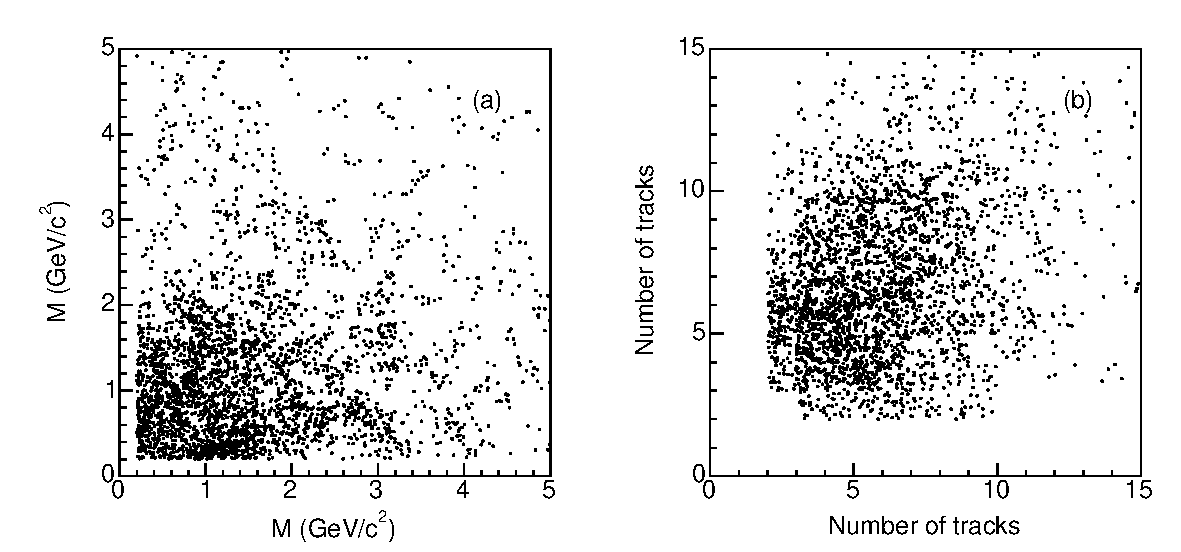
\includegraphics[width=\textwidth]{./figures/MultiMuons2_CDF.pdf}
        %\caption[]{Two-dimensional distributions, reproduced from Ref.~\cite{a0disc},
        %  of (a) the invariant mass, $M$, of all muons and (b) the total
        %  number of tracks contained in a $36.8^{\deg}$ cone when both
        %  cones contain at least two muons.}
      \end{center}
    \end{figure}
    % ========================
    \end{comment}
%  \end{multicols}
\end{multimuons-2}
 \end{column}
%    \end{columns}
%  \end{columns}


%\begin{columns}[t]
%    \begin{columns}[t,totalwidth=1.0\paperwidth] % split up that three-column-wide column
%      \begin{column}{0.35\paperwidth} \begin{MyArticle}[enhanced, tikz={rotate=0}]{Top Quark, Last Piece of Matter, Appears to Be in Place}
  \begin{multicols}{2}
    We establish the existence of the top quark using a 67 pb$^{-1}$ data
    sample of pp collisions at $\sqrt{s} = 1.8$ TeV collected with the Collider
    Detector at Fermilab (CDF). Employing techniques similar to those we
    previously published, we observe a signal consistent with $t\bar{t}$ decay to
    $WWbb$, but inconsistent with the background prediction by
    4.8$\sigma$. Additional evidence for the top quark is provided by a peak in
    the reconstructed mass distribution. We measure the top quark mass
    to be $176 \pm 8 (\text{stat.}) \pm 10 (\text{sys.})$ GeV/c$^{2}$,
    and the $t\bar{t}$ production cross section to be
    $6.8^{+3.6}_{-2.4}$ pb.
    % ========================
    \begin{figure}
      \begin{center}
        \vspace{-0.2in}
        \leavevmode
        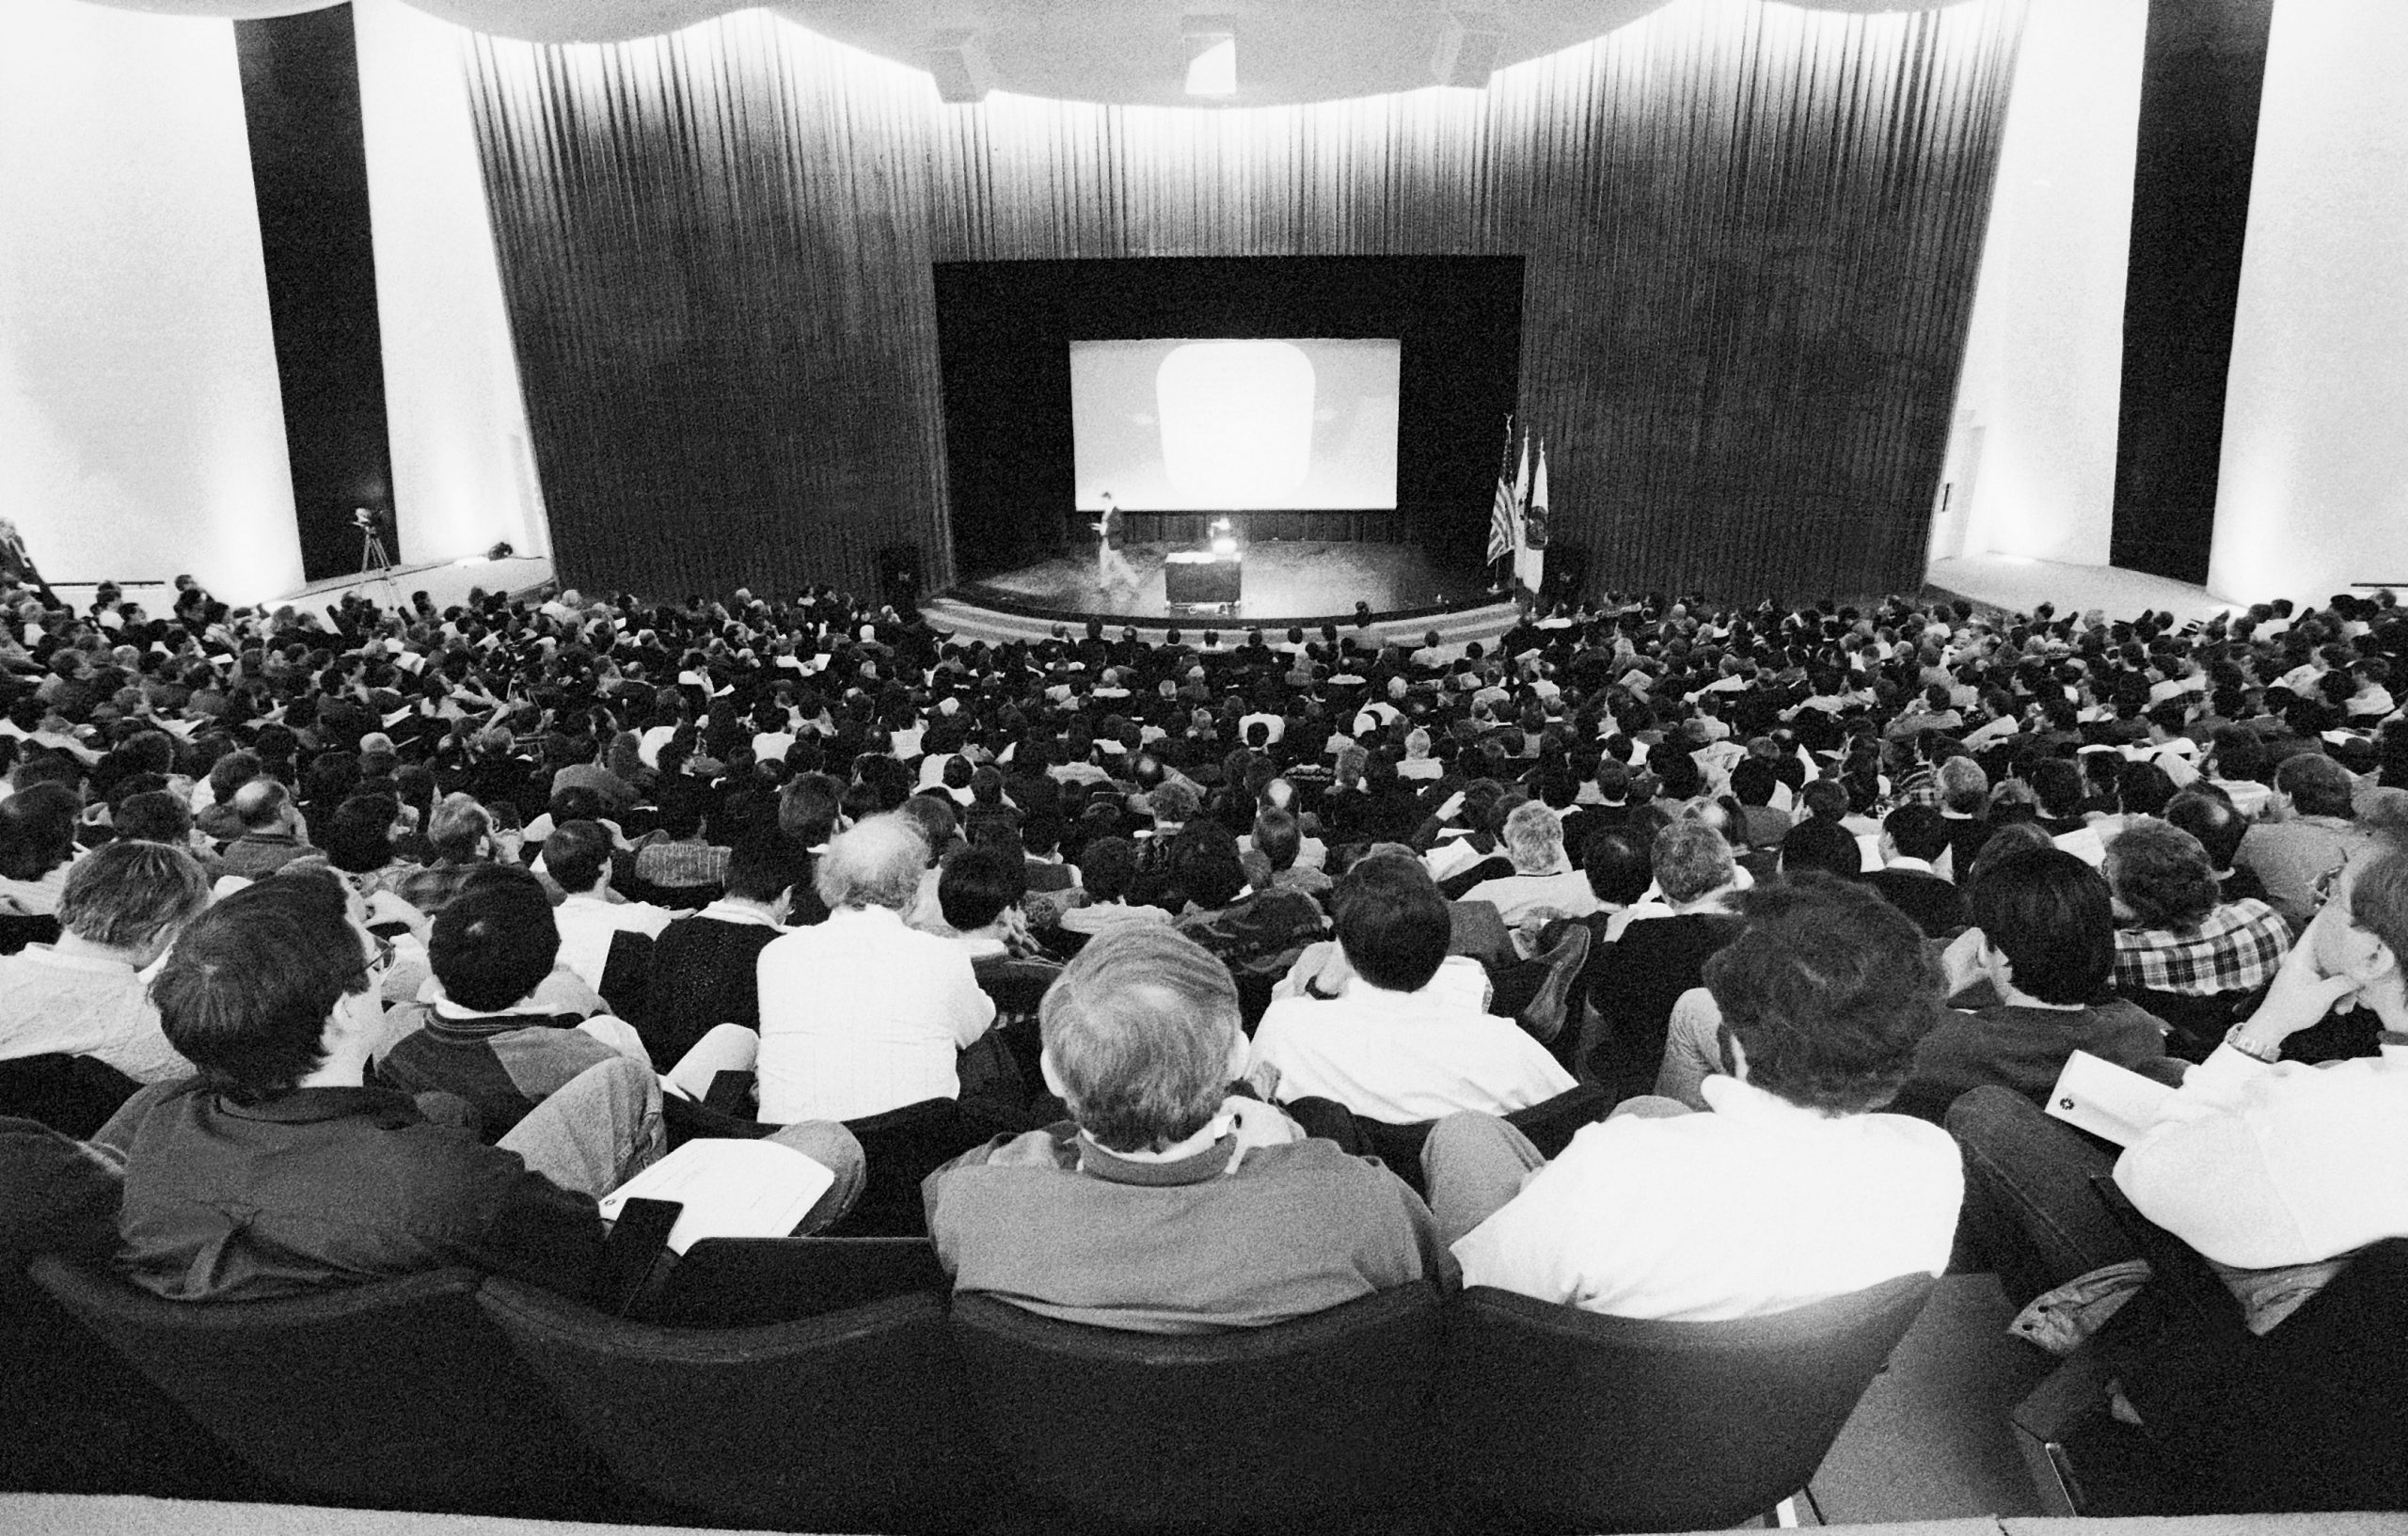
\includegraphics[width=0.5\textwidth]{./figures/TopQuarkAnnouncement.jpg}
      \end{center}
    \end{figure}
    % ========================
  \end{multicols}
\end{MyArticle}
 \end{column}
%      \begin{column}{0.35\paperwidth}  %\begin{MyArticle}[enhanced, height=0.2\textheight,
%tikz={rotate=0}]{Physicists Find Elusive Particle Seen as Key to
%Universe}
\begin{MyArticle}[enhanced, tikz={rotate=0}, width=0.35\textwidth]{Physicists Find Elusive Particle Seen as Key to Universe}
  \begin{multicols}{2}
    Results are presented from searches for the standard model Higgs
    boson in proton–proton collisions at and 8 TeV in the Compact Muon
    Solenoid experiment at the LHC, using data samples corresponding
    to integrated luminosities of up to 5.1 fb$^{−1}$ at 7 TeV and 5.3 fb$^{−1}$
    at 8 TeV. The search is performed in five decay modes:
    $\gamma\gamma$, $ZZ$,  $\tau^{+}\tau^{-}$, and $b\bar{b}$.
    An excess of events is observed above the expected background,
    with a local significance of 5.0 standard deviations, at a mass
    near 125 GeV, signalling the production of a new particle. The
    expected significance for a standard model Higgs boson of that
    mass is 5.8 standard deviations. The excess is most significant in
    the two decay modes with the best mass resolution, $\gamma\gamma$ and $ZZ$; a
    fit to these signals gives a mass of 
    $125.3\pm0.4(\text{stat.})\pm0.5(\text{syst.}$ GeV. The decay to
    two photons indicates that the new particle is a boson with spin 
    different from one. 
    % ========================
    \begin{figure}
      \begin{center}
        \vspace{-0.2in}
        \leavevmode
        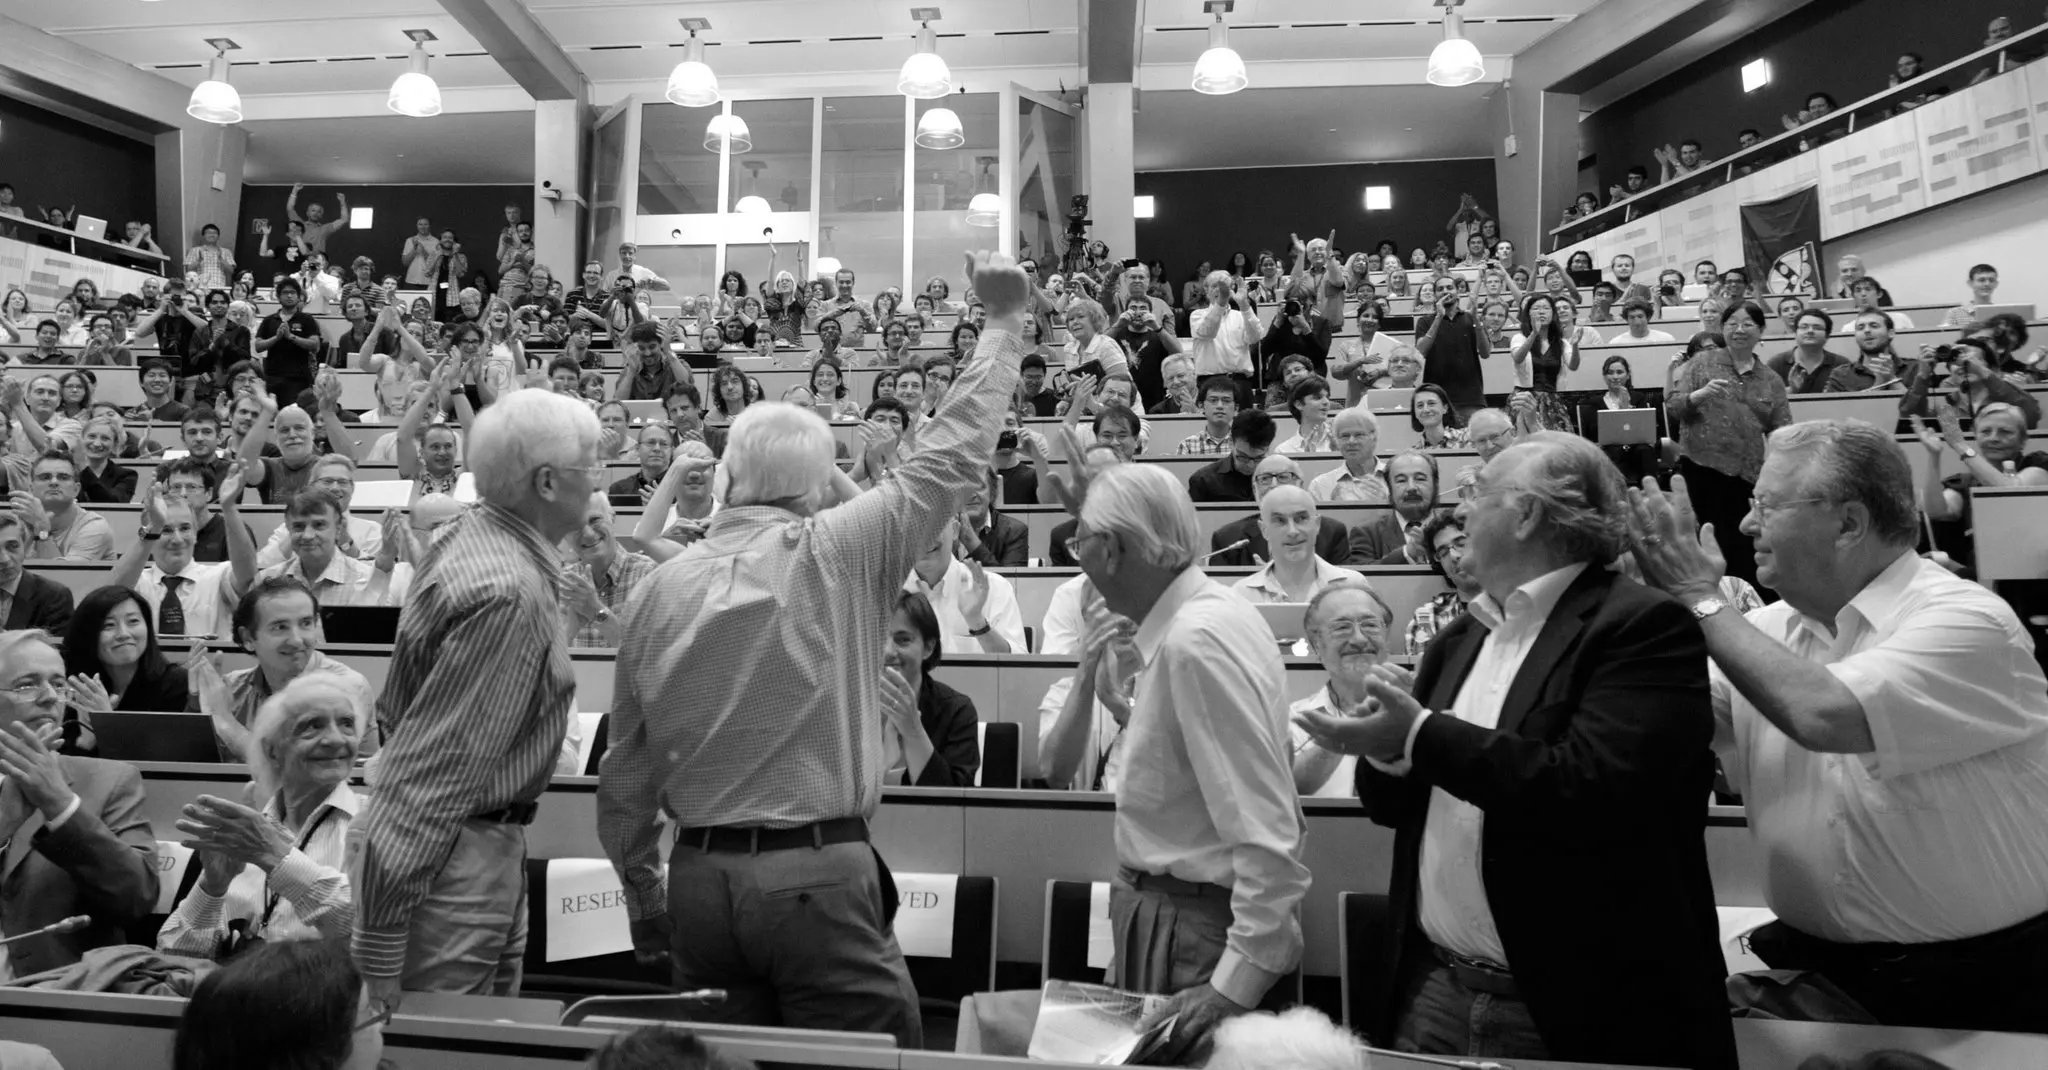
\includegraphics[width=0.5\textwidth]{./figures/HiggsBosonDiscoveryBW.png}
      \end{center}
    \end{figure}
    % ========================
  \end{multicols}
\end{MyArticle}
 \end{column}
%      \begin{column}{0.25\paperwidth} % https://gitlab.cern.ch/tdr/papers/HIG-21-010/-/tree/master/
% new tcolorbox environment
\newtcolorbox{topQuark}[2][]{
  coltext      = black,
  colframe     = \MyBlockFrameColorLeft,
  colback      = \MyBlockFillColorLeft,
  colbacktitle = \MyBlockTitleBoxColor,
  coltitle     = black,
  title        = {\Large{\textbf{#2}}},
  fonttitle    = \bfseries,
  boxrule      = 0.2cm, %frame line width
  %tikz={rotate=#3}, % manipulate the tcolorbox as a whole (in degrees)
  top=+0.0cm, bottom=+0.0cm, left=+0.05cm, right=+0.05cm,
  %enlarge top by   = +1.0cm,  %  equivalent to mdframed 'skipabove'
  %enlarge bottom by= +0.0cm,  %  equivalent to mdframed 'skipbelow'
  %enlarge left by  = +1.5cm,  
  %enlarge right by = +0.0cm, 
  opacityback=1.0, % 1.0 means totally transparent, 0.0 means totally opaque
  arc=0.0cm,        % 0.0cm for non-rounded corners!
  #1,
}

% CMS
\begin{topQuark}[enhanced, tikz={rotate=0}]{Higgs boson: a tool to
    discover new physics: $H^{\pm}$}
  \begin{multicols}{2}
  A search for a charged Higgs boson $H^{\pm}$ decaying
  into a heavy neutral Higgs boson $H$ and a $W$ boson
  is presented. The analysis targets the $W$ decay into a pair
  of tau leptons with at least one of them decaying hadronically and
  with an additional electron or muon present in the event.
  The search is based on proton-proton collision data
  recorded by the CMS experiment during 2016--2018 at
  $\sqrt{s} = 13~TeV$, corresponding to an integrated
  luminosity of 138~$fb^{-1}$. The data are consistent with
  standard model background expectations. Upper limits at 95$\%$ confidence
  level are set on the product of the cross section and branching fraction
  for an $H^{\pm}$ in the mass range of 300--700 GeV, assuming an $H$ 
  with a mass of 200 GeV. The observed limits range from
  0.085 $pb$ for an $H^{\pm}$ mass of
  300 $GeV$ to 0.019~$pb$ for a mass of
  700 $GeV$. These are the first limits on $H^{\pm}$
  production in the $H^{\pm} \to H W^{\pm}$ decay channel at the LHC.
  \end{multicols}
\end{topQuark}
 \end{column}
%    \end{columns}
%  \end{columns}

 

\end{document}

